\documentclass{article}
\usepackage[utf8]{inputenc}
\usepackage[english,russian]{babel} 
\usepackage[a4paper,top=2cm,bottom=2cm,left=3cm,right=1.5cm]{geometry}
\usepackage{amssymb}
\usepackage{esint}
\usepackage{amsmath,amsthm,amssymb}
\usepackage{indentfirst}
\usepackage{hyperref}
\usepackage{csquotes}

\usepackage{abstract}
\renewcommand{\abstractnamefont}{\normalfont\large\bfseries}

\usepackage{minted}
% \RecustomVerbatimEnvironment{Verbatim}{BVerbatim}{}

\usepackage{xcolor}

\usepackage{listings} 
\renewcommand{\listingscaption}{Листинг}

\usepackage{setspace}
\usepackage[nottoc,numbib]{tocbibind}
\usepackage{graphicx}
\usepackage[font=large,justification=centering]{caption}
\usepackage{titlesec}
\usepackage[titletoc]{appendix}
%\usepackage[toc,page]{appendix}

\setstretch{1.35}
\setlength{\abovecaptionskip}{3pt}
\setlength{\parindent}{1.25cm}

\theoremstyle{plain}
\newtheorem{theorem}{Теорема}[section]

\theoremstyle{plain}
\newtheorem{consequence}[theorem]{Следствие}

\theoremstyle{plain}
\newtheorem{lemma}{Лемма}[section]

\theoremstyle{plain}
\newtheorem{claim}{Утверждение}[section]

\theoremstyle{definition}
\newtheorem{definition}{Определение}[section]

\theoremstyle{remark}
\newtheorem{remark}{Замечание}[section]

\theoremstyle{plain}
\newtheorem{exercise}{Упражнение}[section]

\DeclareMathOperator*{\argmin}{arg\,min}
\DeclareMathOperator*{\info}{Info}
\DeclareMathOperator*{\real}{real}
\DeclareMathOperator*{\naive}{naive}
\DeclareMathOperator*{\best}{Best}
\DeclareMathOperator*{\routes}{Routes}
\DeclareMathOperator*{\reduced}{reduced}

\renewcommand{\author}[1]{\def\mtauthortext{#1}}
\renewcommand{\title}[1]{\def\mttitletext{#1}}
\newcommand{\supervisor}[1]{\def\mtsupervisortext{#1}}
\newcommand{\consultant}[1]{\def\mtconsultanttext{#1}}
\newcommand{\groupnum}[1]{\def\mtgroupnumtext{#1}}
\newcommand{\department}[1]{\def\mtdepartmenttext{#1}}
\newcommand{\faculty}[1]{\def\mtfacultytext{#1}}

\renewcommand{\titlepage}{%
    \thispagestyle{empty}
    \begin{center}
    Федеральное государственное автономное образовательное учреждение\break высшего образования\par
    <<Московский физико-технический институт (национальный исследовательский университет)>>\par
    \mtfacultytext{}\par
    \mtdepartmenttext{}\par
\end{center}
%
  {\bf Направление подготовки}: 01.03.02 Прикладная математика и информатика\newline
  {\bf Направленность (профиль) подготовки}: Прикладная математика и компьютерные науки\par
%
  {
\topskip0pt
\vspace*{\fill}
\begin{center}
      {\bf\LARGE \mttitletext{}}\par
      (бакалаврская работа)
\end{center}
\vspace*{\fill}
  }
%
\hfill
\begin{minipage}[t]{7cm}
    {\bf Студент: \newline}
    \mtauthortext{}\newline
\vspace{-3mm}
\rule{7cm}{0.15mm}
\centerline{\small\it (подпись студента)}\newline
    {\bf Научный руководитель: \newline}
    \mtsupervisortext{}\newline
\vspace{-3mm}
\rule{7cm}{0.15mm}
\centerline{\small\it (подпись научного руководителя)}
    {\bf Консультант: \newline}
    \mtconsultanttext{}\newline
\vspace{-3mm}
\rule{7cm}{0.15mm}
\centerline{\small\it (подпись консультанта)}
\end{minipage}
%
\vspace*{\fill}
\begin{center}
      Москва 2021
\end{center}
}

\title{Исследование и оптимизация способов выполнения операции AllReduce в сети в двухуровневой топологией}
\author{Климовицкий Роман Григорьевич}
\supervisor{Звонов Денис Владимирович}
\consultant{Шворин Артем Борисович}
\groupnum{798}
\faculty{Физтех-школа прикладной математики и информатики}
\department{Кафедра банковских информационных технологий}

\begin{document}

\titlepage
\clearpage
\setcounter{page}{2}

\large

\begin{abstract}
\large
    В данной работе рассматриваются различные способы выполнения коллективной операции All\-Re\-duce в сети, имеющей двухуровневую топологию. Целью работы являлось построение отказоустойчивого алгоритма выполнения данной операции, который бы устранял недостатки наивного подхода, основывающегося на коммуникации узлов по принципу \enquote{каждый с каждым}. Основными задачами работы являлись: изучение подходов к реализации AllReduce, построение концепта системы и реализация ее прототипа на языке программирования, формальное доказательство свойств построенного алгоритма. В результате работы был разработан дизайн системы, который позволил снизить затраты ресурсов на сетевую коммуникацию между узлами, а также предоставить ряд гарантий на отказоустойчивость и корректность выполнения операции AllReduce. Основными этапами исследования являлись: рассмотрение подходов к решению задачи и выработка ключевой концепции промежуточных редукций, разработка механизма выбора узлов-редукторов, построение динамической маршрутизации на уровне узлов и реализация AllReduce в соответсвтии с выбранной концепцией. Результаты данной работы могут быть использованы для дальнейшей разработки геораспределенной системы выполнения коллективных операций, а также для ее тестирования и внедрения. В частности, написанный на языке Python прототип (приложение \ref{GitHubLinkAppendix}) может стать отправной точкой для реализации готового продукта.
\end{abstract}
\clearpage

\tableofcontents
\clearpage

\section{Введение}

Типичная инфраструктура компаний, предоставляющих геораспределённые облачные сервисы в интернете (CDN, стримминг видео, публичные VPN, защита от DDoS), представлена в виде набора площадок, где каждая площадка представляет из себя набор вычислительных узлов в пределах одного дата-центра. Связность узлов внутри площадки очень хорошая (малые задержки, большая пропускная способность, высокое качество) и бесплатная, а связность между площадками осуществляется через открытый Интернет, либо арендованные каналы связи, и обладает намного меньшим качеством, которое постоянно варьируется (меняются задержки, процент потерь пакетов, временами связность может пропадать совсем). Важной особенностью является то, что в результате широкого применения в Интернете ECMP-маршрутизации (маршрут выбирается, исходя из значения хэша от адресов источника и получателя пакета), качество связи между узлом $a_1$ площадки $A$ и узлом $b_1$ площадки $B$ может существенно отличаться от качества связи между узлами $a_2$ и $b_2$ тех же площадок. Помимо этого в процессе работы могут добавляться новые узлы и площадки, старые узлы могут выходить из строя, каналы связи могут менять свои качественные характеристики и обрываться.

Иногда для решения различного рода задач, связанных с обработкой данных в описанной инфраструктуре, необходимо поддерживать некоторое когерентное состояние на всех узлах сети, которое достижимо путем применения ассоциативной, коммутативной операции редукции к данным, хранящимся на этих узлах. Например, может потребоваться, чтобы каждый узел знал суммарное количество трафика, обрабатываемое во всей сети.

В настоящее время не существует готового инструмента для решения задач подобного вида, который позволял бы работать с данными большого объема, не страдал от динамического состояния системы и учитывал топологию сети. В данной работе мы изучим возможные подходы для решения поставленной проблемы и при необходимости построим собственный алгоритм для выполнения опсанной операции редукции.

\section{Постановка задачи}

Итак, у нас имеется сеть со следующей топологией: есть несколько площадок, каждая из которых состоит из некоторого количества узлов. Считается, что передача данных между узлами разных площадок — \enquote{дорогая} операция, а внутри площадок — \enquote{почти бесплатная}. Одна из задач данной распределенной системы — сбор некоторых счетчиков с узлов разных площадок и обмен ими для поддержания общего состояния по каждому типу счетчиков. Основной операцией, использующейся в решении этой задачи, является операция AllReduce: после ее завершения каждый узел сети должен узнать результат некоторой редукции по значениям определенного счетчика со всех узлов сети.

Состояние узлов и каналов связи в системе носит динамический характер. В процессе работы могут добавляться новые узлы и площадки, старые узлы могут выходить из строя, каналы связи могут менять свои качественные характеристики и обрываться. Из описанных ограничений формулируется следующая модель отказов, с которой мы далее будем работать. В данной модели отказов возможны следующие отказы оборудования:

\begin{itemize}
    \item Отказ узла (Node failure) — аварийное завершение работы одного узла системы. С некоторого момента времени узел останавливает свою работу без предупреждения, перестает отвечать на запросы и не отправляет никаких сообщений.
    
    \item Отказ канала связи (Link failure) — состояние системы, при котором невозможно доставить сообщение между двумя определенными узлами системы. Может носить временный характер: например, из-за поломки промежуточного сетевого оборудования сетевой инфраструктуре может понадобится некоторое время, чтобы перестроить маршрутизацию.
    
    \item Предполагается, что произвольных (византийских) отказов в системе быть не может: каждый из узлов либо действует строго по заданному протоколу, либо не работает (см. Отказ узла).
\end{itemize}

Помимо всего прочего важным аспектом, который может влиять на множество возможных решений, является набор количественных характеристик системы, в пределах которых она может масштабироваться. Мы будем требовать от нашего решения, чтобы оно работало на стандартном оборудовании при следующих ограничениях:

\begin{itemize}
    \item в сети находится порядка $100$ площадок;
    \item каждая площадка содержит порядка $100$ узлов;
    \item индивидуальные значения счетчиков каждого узла представляют из себя последовательный набор из порядка $10^5$ целых чисел или чисел с плавающей точкой.
\end{itemize}

В простейшей реализации операции AllReduce общение узлов происходит по принципу \enquote{каждый с каждым}, однако этот подход не учитывает высокую стоимость передачи данных между узлами разных групп, а также не соблюдает описанные требования по масштабируемости.

Таким образом, основной целью дальнейшей работы является создание алгоритма для выполнения опреации AllReduce, который бы исправлял недостатки наивного подхода и не страдал от изменчивого состояния системы.

Для достижения поставленной цели выпишем задачи, которые позволят нам к ней приблизиться. Для того, чтобы построить алгоритм, обладающий описанными свойствами, нам необходимо:

\begin{itemize}
    \item изучить возможные способы реализации алгоритма на основе готовых проектов;
    \item построить концепт системы самостоятельно или на основе существующих решений;
    \item формально доказать, что предложенный вариант реализации корректен и обладает необходимыми свойствами;
    \item реализовать прототип системы на одном из языков программирования.
\end{itemize}

Далее опишем соответствующие шаги для выполнения поставленных задач.

\section{Подходы к реализации}

В данном разделе разберем основные подходы для реализации описанной операции AllReduce и выберем среди них наиболее подходящий.

\subsection{All-Reduce из MPI}

В известном интерфейсе для распределенных вычислений MPI (Message Passing In\-ter\-face) есть одноименная операция All-Reduce \cite[стр.~238]{mpi_standard}. Она является аналогом операции Reduce из того же интерфейса с тем отличием, что результат редукции передается всем процессам в группе.

Однако основным недостатком интерфейса MPI является его неустойчивость к отказам процессов. В случае их возникновения текущее выполнение аварийно завершается, и лучшее, что стандартная реализация MPI может предоставить, -- это сообщение о возникшей ошибке и инструменты для ее обработки \cite[стр.~26]{mpi_standard}.

От нашего решения мы будем требовать продолжение работы даже в случае возникновения отказов отдельных узлов. Поэтому мы не будем рассматривать MPI как готовое решение в дальнейшей работе.

\subsection{Согласованное в конечном счете хранилище счетчиков}

Другой вариант реализации, который можно было бы рассматривать, заключается в поддержании согласованной базы счетчиков. Для этого узлам пришлось бы регулярно обмениваться данными индивидуальных счетчиков. В этом случае при необходимости каждый узел сможет проводить редукцию счетчиков, которые он хранит. Этот подход делится на два приципиально отличающихся случая: 1) каждый узел поддерживает хранилище счетчиков всех узлов системы; 2) узел поддерживает базу, состоящию из несобственного подмножества счетчиков. Каждый из случаев также обладает своими недостатками.

В первом случае база счетчиков со всей системы будет занимать в памяти узла достаточно много ресурсов. Если считать, что значение каждого счетчика -- это 64-битное целое число, то для поддержания такого хранилища на каждом узле понадобится около 7-8 ГБ оперативной памяти: всего в сети около $10^4$ узлов, каждый из который обладает набором из $10^5$ счетчиков. Итого, все данные займут около $10^4 \cdot 10^5 \cdot 8\ /\ 1024^3 \approx 7,5$ ГБ. Помимо этого обмен значениями индивидуальных счетчиков между узлами различных площадок не учитывает высокую стоимость передачи данных между ними, поэтому даже в случае поддержания хранилища лишь на подмножестве узлов системы такой метод оказывается слишком требовательным к ресурсам сети и отдельных узлов.

Второй случай в свою очередь не может считаться готовым решением: если разбивать все множество счетчиков на подмножества, необходимо дополнительно продумывать коммуникацию между узлами, обладающими отличными друг от друга данными.

В действительности, хранить \enquote{чужие} индивидуальные счетчики на узлах из-за их быстрого устаревания нецелесообразно. Гораздо разумнее при получении индивидуальных счетчиков другого узла подсчитывать промежуточную редукцию -- благодаря такому подходу можно сохранить память на узлах, а также вместо значений отдельных счетчиков передавать другим узлам сразу результаты частичных редукций. Использование этой идеи обсудим в следующих двух подразделах \ref{NaiveImplementationSubsection} и \ref{GroupReductionSubsection}.

\subsection{Наивная реализация}
\label{NaiveImplementationSubsection}

Как мы уже упоминали, для реализации операции AllReduce можно применить наивный подход, который состоит в попарном общении узлов друг с другом. При использовании этого подхода каждый узел накапливает результат частичной редукции по мере того, как он получает новые значения индивидуальных счетчиков других узлов. Регулярно накопленный результат сохраняется как наиболее актуальный результат операции AllReduce, а затем очищается для подсчета нового.

Несмотря на то, что в данном походе не требуется хранить каждый экземпляр индивидуальных счетчиков отдельно, он все еще страдает от большого объема пересылаемых данных между узлами различных площадок, что опять же не учитывает двухуровневую топологию сети и, более того, в наших ограничениях может оказывать экстремально большую нагрузку на сетевую инфраструктуру.

\subsection{Частичная редукция в пределах площадок}
\label{GroupReductionSubsection}

Прием с подсчетом частичных редукций можно также использовать для того, чтобы сократить сетевую коммуникацию между узлыми разных площадок. Для этого в пределах каждой площадки один или несколько узлов могут накапливать частичную редукцию, состоящую из значений счетчиков узлов данной группы, а затем передавать в другие площадки полученный результат. Поскольку операция редукции ассоциативна, итоговый результат операции AllReduce можно \enquote{собирать} из таких частичных редукций вместо добавления каждого индивидуального счетчика по отдельности. Коль скоро вся коммуникация между площадками, относящаяся к непосредственной реализации операции AllReduce, в данном подходе будет состоять лишь из передачи результатов промежуточных редукций, он будет заведомо эффективнее наивного подхода. Поэтому мы возьмем описанную идею за основу, на которой будет строиться дальнейшее наше решение.

\section{Математическая постановка задачи}

Перед тем, как приступать к описанию алгоритма, введем формальные обозначения и сформулируем задачу в новых терминах. Это необходимо для задания четких требований к реализации. Зафиксированные обозначения нам также помогут ясно выражать утверждения при доказательстве тех или иных свойств построенной системы.

\subsection{Двухуровневая топология сети}

\begin{definition}
    Пусть \textit{$S$ – множество всех узлов сети}. \textit{Узлом сети} будем называть любой элемент множества $S$. За $N := |S|$ обозначим количество узлов в сети.
\end{definition}

\begin{definition}
    Изначально все узлы разбиты на непересекающиеся множества $S_1, S_2, \ldots, S_n$, называемые \textit{площадками}. $\mathcal{S} := \{S_1, \ldots, S_n\}$ -- \textit{множество всех площадок}.
\end{definition}

Таким образом, выполнено: $\displaystyle \bigsqcup_{k = 1}^n S_k = S$. Для простоты будем считать, что все площадки не пустые: $\forall k\ S_k \neq \varnothing$.

\subsection{Метрика сети}

В дальнейшем мы будем работать с сущностями, которые со временем могут изменяться. Поэтому зафиксируем понятие временной шкалы, с которой мы далее будем работать, чтобы отразить динамическую природу решаемой задачи:

\begin{definition}
    $T \in \{\mathbb{R}_+,\ \mathbb{Z}_+\}$ -- \textit{шкала времени}.
\end{definition}

\begin{definition}
    Каждый из узлов $a \in S$ имеет доступ к некоторой \textit{динамической информации} $\info_t(a, b) \in I_d$ о качестве непосредственного соединения до всех других узлов $b \in S \setminus \{a\}$, т.е. $\{\info_t\}_{t \in T}$ -- семейство частично определенных, индексированных параметром времени функций вида $\info_t: S \times S \to I_d$.
\end{definition}

\begin{definition}
\label{MetricDefinition}
    По динамической информации информации считается \textit{метрика качества соединения} $m: I_d \to \mathbb{R}_{>0}$. При этом можем определить \textit{метрику непосредственного соединения между узлами $a$ и $b$ в момент времени $t$} $m_t: S \times S \to \mathbb{R}_+$ так, что
    \[ m_t(a, b) :=
      \begin{cases}
        m(\info_t(a, b)) &,\ a \neq b \\
        0 &,\ a = b
      \end{cases}
    \].
\end{definition}

\begin{remark}[Физический смысл метрики]
\label{MetricPhysicalMeaning}
    В понятие динамической информации может входить целый ряд свойств канала связи: как статических (стоимость передачи данных по данному каналу, его приоритет), так и динамических (RTT \cite{definition:round-trip_delay_time}, потеря пакетов \cite{RFC1242}, явный флаг о работоспособности канала). \enquote{Хорошая} функция метрики качества должна учитывать природу этих данных и отражать реальное качество сетевого соединения: чем ниже метрика, тем выше характеристики канала в совокупности. В том числе, если узел $b$ неработоспособен в момент времени $t$, то до него невозможно доставить данные, а значит и $\forall a \in S \setminus \{ b \}$ значения $m_t(b, a)$ и $m_t(a, b)$ должны быть бесконечно большими по сравнению с метрикой соединения между любыми другими рабочими узлами. Известно \cite{networking:best-effort-service}, что в сетевой инфраструктуре нельзя гарантировать доставку данных за ограниченное время. Однако хотелось бы иметь некоторую уверенность в том, что при достаточно низкой метрике вероятность неуспешной передачи данных стремится к нулю -- \enquote{хорошая} функция метрики должна учитывать и эту особенность сети. Тем не менее, в данной работе мы абстрагируемся от явного вида данной функции, чтобы сосредоточиться на основной цели по оптимизации выполнения операции AllReduce.
\end{remark}

Определение метрики соединения \ref{MetricDefinition} вполне естественно: нам ничего не стоит передать данные самому себе, ведь они у нас уже есть, но при этом мы не можем отправить данные кому-то другому совсем бесплатно.

\begin{remark}
\label{MetricEmpiricalRule}
    Считается, что почти всегда выполнено следующее: 
    \[
        \forall\ i,\ j,\ k \in \{1,\ \ldots,\ n\}\ ( i \neq j \implies \forall\ a \in S_i,\ b \in S_j,\ c \in S_k,\ d \in S_k\ m_t(a, b) \gg m_t(c, d))
    \] -- метрика соединения между узлами разных площадок существенно выше метрики соединения между узлами одной площадки.
\end{remark}

\subsection{Операция AllReduce}

Считается, что у каждого узла системы есть изменяющиеся со временем счетчики. Глобальная задача заключается в применении редуцирующей коммутативной ассоциативной операции к значениям счетчиков всех узлов и распространении результата на все узлы системы. Узлы способны выполнять частичную редукцию полученных от других узлов счетчиков и отправлять полученный промежуточный результат другим узлам. Они также способны применять операцию к полученным частичным результатам.

\begin{definition}
    Описанная глобальная операция называется \textit{AllReduce}.
\end{definition}

\begin{definition}
    Введем обозначения:
    \begin{itemize}
        \item $C$ -- универсум значений счетчиков и результатов их редукций, которыми владеют узлы системы;
        \item $c_t : S \to C$ -- функция, возвращающая значение счетчиков определенного узла в момент времени $t$;
        \item $|\cdot| : C \to \mathbb{N}$ -- функция, возвращающая размер элемента множества счетчиков в единицах памяти, аналог объема пересылаемых данных;
        \item $+ : C \times C \to C$ -- операция редукции;
        \item $\displaystyle \sum_{i = k}^k c_i := c_k,\ \displaystyle \sum_{i = k}^m c_i := \displaystyle \sum_{i = k}^{m - 1} c_i + c_m,\ k \neq m,\ \forall i \in \mathbb{N}\ c_i \in C$ -- семейство операторов различной валентности для краткой записи редукции, примененной несколько раз;
        \item $0 \in C$ -- нейтральный элемент по операции редукции: $\forall c \in C\ c + 0 = 0 + c = c$.
    \end{itemize}
\end{definition}

Мы используем знаки \enquote{плюса} и суммирования для наглядности -- операция сложения, как правило, коммутативная и ассоциативная, а сумма счетчиков -- один из возможных результатов редукции, который необходимо получить в конце выполнения AllReduce. Также для удобства будем использовать инфиксную запись.

Поскольку коммуникация между узлами может занимать любой положительный отрезок времени, отправляемые данные могут произвольным образом терять свою актуальность до ее завершения. Значит любое доступное нам решение не может гарантировать того, что результат работы алгоритма будет всегда равен результату редукции, примененной к актуальным значениям счетчиков. Тем не менее, мы можем требовать более слабых гарантий от решения -- для этого определим, что мы будем считать корректным выполнением операции AllReduce.

\begin{definition}
\label{AllReduceСorrectness}
    Пусть узел $a \in S$ в момент времени $t \in T$ локально завершил выполнение операции AllReduce и в качестве результата получил значение $c_{AR}$. Для каждого узла $a_i \in S$ рассмотрим множество $C_i = \{ c_t(a_i) : t \in [t - \Delta, t] \} \subset C$ из значений индивидуальных счетчиков данного узла, которыми он владел в разные моменты на временном отрезке $[t - \Delta, t]$. В частности, если узел $a_k$ в данный промежуток времени не работал или находился в недоступной части сети, будем считать $C_k = \{ 0 \}$. Результат операции AllReduce $c_{AR}$ будем называть \textit{корректным с допустимым временным отклонением $\Delta > 0$}, если $\exists \{ c_i \}_{i = 1}^N : \forall i \leq N\ c_i \in C_i \wedge c_{AR} = \displaystyle \sum_{i = 1}^N c_i$.
\end{definition}

\begin{remark}
    В частности, если с некоторого момента времени значения счетчиков на узлах перестали меняться, корректная в наших терминах реализация операции AllReduce за ограниченное время должна привести к тому, что результаты редукции на узлах будут согласованы в пределах каждой компоненты сильной связности сети.
\end{remark}

Перейдем к формальной постановке задачи по снижению суммарной стоимости выполнения операции AllReduce.

\begin{remark}
\label{ReductionOptimization}
    Считается, что верно следующее: $\forall\ c_1, c_2 \in C\ |c_1 + c_2| \leq |c_1| + |c_2|$, т.е. промежуточная редукция не увеличивает размер передаваемых данных.
\end{remark}

\begin{definition}
\label{CostFunctionDefinition}
    Пусть функция $cost : \mathbb{R}_{+} \times \mathbb{Z}_{+} \to \mathbb{R}_{+}$ обладает следующими свойствами:
    \begin{enumerate}
        \item $\forall\ l \in \mathbb{Z}_{+}\ cost(0, l) = 0$;
        
        \item $\forall\ m \in \mathbb{R}_{+}\ cost(m, 0) = 0$;
        
        % \item монотонность по первому аргументу: $\forall\ l \in \mathbb{Z}_{+}\ \forall\ m_1, m_2 \in \mathbb{R}_{+}\ (m_1 < m_2 \implies cost(m_1, l) < cost(m_2, l))$;
        
        \item $\forall\ l \in \mathbb{Z}_{+}\ \forall\ m_1^{(1)}, m_2^{(1)}, \ldots, m_p^{(1)}, m_1^{(2)},\ m_2^{(2)}, \ldots, m_q^{(2)} \in \mathbb{R}_{+}$ 
        
        \begin{equation*}
            \Big( \displaystyle \sum_{i = 1}^p m_i^{(1)} < \displaystyle \sum_{j = 1}^q m_j^{(2)} \implies \displaystyle \sum_{i = 1}^p cost(m_i^{(1)}, l) < \displaystyle \sum_{j = 1}^q cost(m_j^{(2)}, l) \Big);
        \end{equation*}
        
        \item монотонность по второму аргументу: $\forall\ m \in \mathbb{R}_{+}\ \forall\ l_1, l_2 \in \mathbb{Z}_{+}\ (l_1 < l_2 \implies cost(m, l_1) < cost(m, l_2))$.
    \end{enumerate}
    Тогда $cost$ называется \textit{функцией стоимости передачи данных}.
\end{definition}

\begin{definition}
    Пусть $cost$ -- некоторая функция стоимости передачи данных, $t \in T,\ a, b \in S,\ l \in \mathbb{N}$. Величину $cost_t(a, b, l) := cost(m_t(a, b), l)$ назовем \textit{стоимостью передачи данных объемом $l$ по каналу связи $(a, b)$ относительно $cost$ в момент времени $t$}.
\end{definition}

\begin{definition}
    Пусть $cost$ -- некоторая функция стоимости передачи данных, $t \in T,\ a, b \in S,\ c \in C$. Величину $cost_t(a, b, c) := cost_t(a, b, |c|)$ назовем \textit{стоимостью передачи счетчиков $c$ относительно $cost$ из узла $a$ в узел $b$ в момент времени $t$}.
\end{definition}

Ставится задача снижения суммарной стоимости передачи данных, необходимой для корректного выполнения операции AllReduce с ограниченным допустимым временным отклонением. Из замечаний \ref{MetricEmpiricalRule} и \ref{ReductionOptimization} возникает предложение проводить частичную редукцию счетчиков одной площадки на небольшом числе узлов данной площадки и передавать полученный результат в другие площадки для подсчета окончательного результата.

Для реализации предложенного механизма каждый из узлов должен быть способен выполнять следующие задачи:

\begin{enumerate}
    \item Определять узел своей площадки, на который он передаст данные своих счетчиков для последующей редукции и отправки;
    
    \item Отправлять данные на узлы других площадок таким образом, чтобы суммарная стоимость их передачи была минимальна;
    
    \item Накапливать результаты промежуточных редукций: как внутри площадки, так и промежуточные результаты, пришедшие с других площадок.
\end{enumerate}

Первый пункт из списка решим посредством введния узлов-редукторов, которые будут определяться аналогично выбору DR и BDR из протокола OSPF \cite[стр.~75]{RFC2328} -- на них же мы в будущем сможем хранить произвольные данные, отражающие состояние площадки. В разделе \ref{ReducersSection} сформулируем алгоритм, по которому данный выбор происходит. Реализацию второго пункта обеспечим введением собственного протокола маршрутизации на уровне узлов сети, который опишем в следующем разделе \ref{RoutingSection}. Третий пункт, являющийся завершающим в подсчете результата AllReduce, раскроем в соответствующем разделе \ref{AllReduceSection}.

\section{Узлы-редукторы}
\label{ReducersSection}

Основной целью данного раздела будет являться построение алгоритма, позволяющего определить в пределах каждой площадки единственный узел для централизованного выполнения операции редукции на нем.

\subsection{Существующие решения}

В мире существуют несколько подходов к решению задачи выбора лидера, которые отличаются предоставляемыми гарантиями. Мы рассмотрим два из них, которые имеют широкое применение в современных распределенных системах: выбор лидера в RAFT \cite{RAFT} и выбор DR и BDR в OSPF  \cite[стр.~75]{RFC2328}.

Алгоритм выбора лидера RAFT гарантирует, что в пределах работающего кластера ни в один момент времени не будет присутствовать более одного лидера. Зачастую данное свойство очень полезно при проектировании систем, в которых важна консистентность. Однако это также накладывает ограничения на доступность системы при разделении сети: меньшая часть кластера не может выбирать нового лидера из-за того, что для перехода в состояние лидерства узлу необходимо получить подтверждение хотя бы у половины узлов сети. С этим же связана другая его особенность: в процессе работы могут возникать \enquote{несостоявшиеся} выборы, когда ни один из узлов не набрал необходимый кворум. Чтобы с этим бороться, в RAFT используется прием случайных временных интервалов между посылкой сообщений. Однако с увеличением числа узлов, участвующих в выборах, стоит ожидать, что многие узлы будут инициировать новые выборы примерно в одно время, что приведет к частым перезапускам данной процедуры. Увеличение числа узлов приводит также к сокращению средней продолжительности эпохи, в которой определен лидер, что было описано и доказано в работе \cite{RAFT_performance_1808.01081}. Тем не менее, все эти ограничения оправданы -- на основе данного алгоритма в RAFT строится распреденный журнал, который требует высокой степени согласованности.

Другой алгоритм выбора единого узла, который мы рассмотрим, описывается в формате выбора Designated Router (DR) и Backup Designated Router (BDR) в протоколе динамической маршрутизации OSPF \cite[стр.~75]{RFC2328}. Он обладает более слабыми гарантиями по сравнению с предыдущим решением и допускает наличия временных промежутков, когда описанный выбор не согласован. Данный алгоритм опирается на предопределенную информацию о том, что при прочих равных выбранный узел определяется однозначно в соответствии со статической информацией. Это позволяет узлам эффективно разрешать конфликты, а также \enquote{предсказывать} исход выборов неявно и заранее. Таким образом, данный алгоритм позволяет всем узлам действовать асинхронно, что повышает доступность системы в ущерб согласованности, а также позволяет зайдействовать в алгоритме относительно большое количество узлов. Несмотря на отсутствие гарантий по согласованности, выбор резервного узла не делает отказ текущего \enquote{лидера} критичным -- в данном случае резервный узел перенимает его ответственность на себя, что в том числе позволяет поддерживать некоторое состояние кластера, например, текущий результат редукции.

С учетом всего вышесказанного было принято решение использовать алгоритм выбора DR и BDR в OSPF в качестве основной идеи для выбора наших узлов-редукторов, поскольку он больше всего подходит под наши задачи: мы не требуем жесткой согласованности в выборе единых узлов и готовы мерится с короткими промежутками времени, когда их может быть несколько. Более того, использование данного решения позволит работать всем узлам по одному и тому же механизму и не заботится об их количестве. В случае консенсусного выбора лидера пришлось бы ограничивать набор узлов, на котором он бы выполнялся.

\subsection{Алгоритм выбора узла-редуктора}
\label{ReducersElectionSubsection}

Опишем непосредственно алгоритм, по которому каждый из узлов будет определять текущий узел-редуктор.

Здесь и далее в работе будем описывать различные сообщения, которыми узлы будут обмениваться, в формате protobuf-сообщений из фреймворка Google Protocol Buffers \cite{Google_protobuf}, который позволяет сериализовать и десериализовать данные, предназначенные для отправки по сети.

Заведем таймер, по которому каждый узел один раз в промежуток времени $\Delta_{hb}$ будет отправлять всем узлам собственной площадки heartbeat-сообщения вида, представленного в листинге \ref{lst:HeartbeatMessage}.

\begin{listing}[!htb]
\begin{minted}
[
frame=lines,
framesep=2mm,
baselinestretch=1.2,
fontsize=\normalsize,
% numbersep=-2pt,
linenos
]
{proto}
message HeartbeatMessage {
    NeighbourState state = 1;
    uint64 start_ts = 2;
}
\end{minted}
\caption{Описание heartbeat-сообщения в формате protobuf-сообщения.}
\label{lst:HeartbeatMessage}
\end{listing}

В данном сообщении \texttt{NeighbourState} -- это protobuf-перечисление из листинга \ref{lst:NeighbourState}.

\begin{listing}[!htb]
\begin{minted}
[
frame=lines,
framesep=2mm,
baselinestretch=1.2,
fontsize=\normalsize,
linenos
]
{proto}
enum NeighbourState {
  OTHER = 0;
  REDUCER = 1;
  BACKUP_REDUCER = 2;
}
\end{minted}
\caption{Protobuf-перечисление из возможных состояний узла.}
\label{lst:NeighbourState}
\end{listing}

Мы хотим добиться того, чтобы каждый из узлов площадки в каждый момент времени, возможно неявно, находился в одном из состояний \texttt{REDUCER}, \texttt{BACKUP\_REDUCER} и \texttt{OTHER} и данную информацию вместе со временем начала работы указывал в своих heartbeat-сообщениях. Для этого на каждом из узлов зведем переменные \texttt{reducer} и \texttt{backup\_reducer}, которые будут содержать идентификаторы узлов, которых данный узел считает редуктором и резервным редуктором соответственно, а также последние полученные от них времена начала работы. Таким образом, эти поля будут иметь тип \texttt{NeighbourRevision} (листинг \ref{lst:NeighbourRevision}).

\begin{listing}[!htb]
\begin{minted}
[
frame=lines,
framesep=2mm,
baselinestretch=1.2,
fontsize=\normalsize,
linenos
]
{python}
class NeighbourRevision:
    def __init__(self, node_id: int, start_ts: int):
        self.id = node_id
        self.start_ts = start_ts
\end{minted}
\caption{Определение класса \texttt{NeighbourRevision}.}
\label{lst:NeighbourRevision}
\end{listing}

Путем добавления к идентификатору узла отметки времени начала его работы мы можем перейти к новой модели отказов, в которой все отказавшие узлы никогда не перезапускаются вновь, а вместо них запускаются новые узлы с новой отметкой времени. Действительно, таким образом, пары \enquote{идентификатор-временная отметка} для каждого запуска узла будут уникальными.

Изначально полям \texttt{reducer} и \texttt{backup\_reducer} присвоим значения \texttt{Neigh\-bour\-Re\-vi\-si\-on(-1, -1)}, что будет означать, что узел не обладает информацией о том, кто в данный момент является редуктором и резервным редуктором. Значения данных полей определяют состояние, в котором находится данный узел, которое будет добавлено в его heartbeat-сообщение. Если идентификатор самого узла равен значению идентификатору одного из данных полей, его состояние определяется соответствующим образом, описанным в листинге \ref{lst:ReducerGetState}.

\begin{listing}[!htb]
\begin{minted}
[
frame=lines,
framesep=2mm,
baselinestretch=1.2,
fontsize=\normalsize,
linenos
]
{python}
def __get_state(self) -> reduction_pb2.NeighbourState.V:
    if self.__reducer.id == self.__id:
        return REDUCER
    elif self.__backup_reducer.id == self.__id:
        return BACKUP_REDUCER
    else:
        return OTHER
\end{minted}
\caption{Определение состояния узла по значениям его полей \texttt{reducer} и \texttt{backup\_reducer}.}
\label{lst:ReducerGetState}
\end{listing}

При этом будем стремится к тому, чтобы как можно чаще выполнялись следущие условия:

\begin{itemize}
    \item Ни один из узлов не должен считаться редуктором и резервным редуктором одновременно.

    \item При условии отсутствия разделения сети \cite[стр.~2]{CAP_Theorem} внутри площадки в один момент времени на ней не должно быть больше одного узла, которого хотя бы один работающий узел считал бы редуктором. Аналогично для резервных редукторов.
    
    \item Если на площадке есть хотя бы один рабочий узел, редуктор должен быть выбран на каждом из узлов. Если на площадке есть хотя бы два рабочих узла, на каждом из них должны быть выбраны и редуктор, и резервный редуктор.
    
    \item В случае отказа редуктора новым редуктором должен стать текущий резервный редуктор. Соответственно, резервный редуктор должен переизбраться.
\end{itemize}

Для выполнения условия на единственность редуктора и резервного редуктора заведем правило, по которому будут разрешаться конфликты: если узлу $a$ приходит heartbeat-сообщение от узла $b$ со значением \texttt{state}, равным \texttt{REDUCER}, а идентификатор узла $b$ больше значения поля \texttt{reducer.id} у узла $a$, то данному полю присваивается новое значение, равное идентификатору узла $b$. Если при этом значения \texttt{reducer} и \texttt{backup\_reducer} стали равны, значение \texttt{backup\_reducer} инвалидируется. Аналогично для резервного редуктора с тем лишь отличием, что мы ничего не делаем, если heartbeat-сообщение пришло от узла, которого мы в данный момент считаем редуктором (такая ситуация может возникнуть, когда резервный редуктор еще не успел понять, что сам должен заменить редуктора, но должен отправить очередное heartbeat-сообщение). Нам также важно обновить временную отметку текущих узлов на актуальную, если она изменилась. Если же пришедшее heartbeat-сообщение имеет поле \texttt{heartbeat.state}, равное \texttt{OTHER}, и оно было отправлено текущим редуктором или резервным редуктором с изменением временной отметки, значит данный узел перезапустился и мы обладаем неактуальной информацией и ее также необходимо инвалидировать. Стоит отметить, что здесь важную роль играет временная отметка узла: с ее помощью мы отличаем ситуацию, когда назначенный редуктор или резервный редуктор отказал от той, когда он сам еще не узнал, в каком состоянии он находится.

Таким образом, при возникновении конфликтов больший приоритет в выборе редуктора или резервного редуктора имеет узел с большим идентификатором. При условии надежной сети (отсутствие потерь, минимальные задержки) такое правило сможет нам гарантировать, что с момента возникновения несогласованности в виде разных редукторов (резервных редукторов) на одной площадке при отсутствии дальнейших отказов узлов пройдет не больше $\Delta_{hb}$ времени до наступления момента, когда выбор редуктора (резервного редуктора) станет согласован. Помимо всего прочего, введенное правило в дальнейшем будет влиять на алгоритм выбора редуктора и резервного редуктора при обнаружении отказов.

Другая особенность, которую стоит учитывать при получении heartbeat-сообщения от текущего редуктора или резервного редуктора, заключается в том, что данное сообщение может содержать информацию, не согласующуюся с текущими значениями полей \texttt{reducer} и \texttt{backup\_reducer}. Например, такая ситуация может возникнуть в случае, когда редуктор отказал, текущий узел заметил это и в качестве редуктора установил значение текущего резервного редуктора $b$, но сам узел $b$ об этом еще не узнал и, продолжая считать себя резервным редуктором, отправил текущему узлу heartbeat-сообщения. Для того, чтобы не инвалидировать значение редуктора в данном случае, заведем поля \texttt{redcuer\_till\_expiration} и \texttt{backup\_till\_expiration}, которые при каждом обновлении редуктора или резервного редуктора будут устанавливаться равными $n_e$ (можно считать $n_e = 1$). В дальнейшем будем использовать эти поля для отличия штатных ситуаций от неполадок, в процессе чего их значения могут уменьшаться. При получении heartbeat-сообщения с ожидаемым состоянием будем возвращать исходное значение $n_e$.

Итоговый код обработки heartbeat-сообщения представлен в листинге \ref{lst:HandleHeartbeat}.

\begin{listing}[!htb]
\begin{minted}
[
frame=lines,
framesep=2mm,
baselinestretch=1.2,
fontsize=\normalsize,
linenos
]
{python}
def handle_heartbeat(self,
                     heartbeat: reduction_pb2.HeartbeatMessage,
                     source_node: int) -> None:
    self.__received_heartbeats[source_node] = heartbeat
    source_revision = NeighbourRevision(source_node, heartbeat.start_ts)
    if heartbeat.state == REDUCER:
        if self.__reducer.id < source_revision.id or \
                self.__is_new_revision(self.__reducer, source_revision):
            self.__set_reducer(source_revision)
            if self.__reducer.id == self.__backup_reducer.id:
                self.__set_backup(NeighbourRevision(-1, -1))
        elif self.__is_same(self.__reducer, source_revision):
            self.__reducer_till_expiration = self.__STATE_EXPIRATION
    elif heartbeat.state == BACKUP_REDUCER:
        if self.__is_same(self.__reducer, source_revision):
            return
        if self.__backup_reducer.id < source_revision.id or \
                self.__is_new_revision(self.__backup_reducer, source_revision):
            self.__set_backup(source_revision)
        elif self.__is_same(self.__backup_reducer, source_revision):
            self.__backup_till_expiration = self.__STATE_EXPIRATION
    elif heartbeat.state == OTHER:
        if self.__is_new_revision(self.__reducer, source_revision):
            self.__set_reducer(NeighbourRevision(-1, -1))
        elif self.__is_new_revision(self.__backup_reducer, source_revision):
            self.__set_backup(NeighbourRevision(-1, -1))
\end{minted}
\caption{Обработка приходящих heartbeat-сообщений.}
\label{lst:HandleHeartbeat}
\end{listing}

В реализации описанного метода используются вспомогательные функции для различных проверок, код которых представлен в листинге \ref{lst:RevisionsComparison}.

\begin{listing}[!htb]
\begin{minted}
[
frame=lines,
framesep=2mm,
baselinestretch=1.2,
fontsize=\normalsize,
linenos
]
{python}
@staticmethod
def __is_new_revision(prev: NeighbourRevision, cur: NeighbourRevision) -> bool:
    return prev.id == cur.id and prev.start_ts < cur.start_ts

@staticmethod
def __is_same(node_1: NeighbourRevision, node_2: NeighbourRevision) -> bool:
    return node_1.id == node_2.id and node_1.start_ts == node_2.start_ts
\end{minted}
\caption{Вспомогательные функции для проверки актуальности имеющихся данных о редукторе и резервном редукторе.}
\label{lst:RevisionsComparison}
\end{listing}

Для определения отказов узлов заведем еще один таймер с временным интервалом $\Delta_{dead}$. Несмотря на то, что по замечанию \ref{MetricEmpiricalRule} качество сети в пределах площадки достаточно хорошее, даже между рабочими узлами единичные пакеты могут терятся или соединение может временно иметь высокую задержку. Поэтому, чтобы свести к минимуму число ситуаций, когда рабочий узел считается отказавшим из-за проблем сети, $\Delta_{dead}$ должен превосходить $\Delta_{hb}$ в несколько раз. Для определенности возьмем $\Delta_{dead} = 3\Delta_{hb}$. В промежутках между срабатываниями таймера по детекции отказов будем сохранять последние heartbeat-сообщения от каждого из узлов в хэш-таблицу \texttt{re\-cei\-ved\_heart\-beats}, перед запуском нового таймера данную таблицу будем очищать. Отказавшими будем считать те узлы, от которых за очередной промежуток времени $\Delta_{dead}$ мы не получили ни одного heartbeat-сообщения. Если среди таких узлов оказался хотя бы один из узлов с идентификаторами \texttt{reducer} и \texttt{backup\_reducer}, либо же последние heartbeat-сообщения говорят о том, что состояние кого-то из них давно (на протяжении $n_e \cdot \Delta_{dead}$ времени) не согласуется текущими значениями данных полей, то запускается алгоритм перевыборов (метод \texttt{reelect}). Последняя проверка будет осуществляться следующим образом: если при очередном срабатывании таймера $\Delta_{dead}$ состояние последнего полученного heartbeat-сообщения от узла, которого мы считаем редуктором, не равно \texttt{REDUCER}, уменьшаем значение поля \texttt{reducer\_till\_expiration} на 1. Если значение \texttt{reducer\_till\_expiration} стало отрицательным, значит состояние узла давно не согласуется с ожиданиями и нужно запустить алгоритм перевыборов. Аналогично для резервного редуктора.

Итого, каждый промежуток времени в $\Delta_{dead}$ мы будем запускать следующую процедуру:

\begin{listing}[!htb]
\begin{minted}
[
frame=lines,
framesep=2mm,
baselinestretch=1.2,
fontsize=\normalsize,
linenos
]
{python}
def __check_availability(self) -> None:
    if not self.__is_node_alive(self.__reducer) or \
            not self.__is_node_alive(self.__backup_reducer):
        self.__reelect()
    else:
        if not self.__is_in_state(self.__reducer.id, REDUCER):
            self.__reducer_till_expiration -= 1
        if not self.__is_in_state(self.__backup_reducer.id, BACKUP_REDUCER):
            self.__backup_till_expiration -= 1
        if self.__reducer_till_expiration < 0 or \
                self.__backup_till_expiration < 0:
            self.__reelect()

    self.__received_heartbeats.clear()

def __is_node_alive(self, node: NeighbourRevision) -> bool:
    return node.id in self.__received_heartbeats and \
           node.start_ts == self.__received_heartbeats[node.id].start_ts

def __is_in_state(self,
                  node_id: int,
                  required_state: reduction_pb2.NeighbourState.V) -> bool:
    if node_id not in self.__received_heartbeats:
        return False
    return self.__received_heartbeats[node_id].state == required_state
\end{minted}
\caption{Проверка работоспособности редуктора и резервного редуктора по набору полученных heartbeat-сообщений.}
\label{lst:CheckAvailability}
\end{listing}

Сам алгоритм перевыборов (метод \texttt{reelect}) опишем последовательно по шагам:

\begin{enumerate}
    \item Если среди отказавших или несогласованных узлов есть \texttt{reducer}, ставим на его место текущий \texttt{backup\_reducer} и инвалидируем \texttt{backup\_reducer} (листинг \ref{lst:CheckReducer}).
    
\begin{listing}[!htb]
\begin{minted}
[
frame=lines,
framesep=2mm,
baselinestretch=1.2,
fontsize=\normalsize,
linenos
]
{python}
if not self.__is_node_alive(self.__reducer) or \
        self.__reducer_till_expiration < 0:
    self.__set_reducer(self.__backup_reducer)
    self.__set_backup(NeighbourRevision(-1, -1))
\end{minted}
\caption{Проверка работоспособности текущего редуктора.}
\label{lst:CheckReducer}
\end{listing}

    \item Определяем множество доступных узлов $A$ как множество ключей хэш-таблицы \texttt{received\_heartbeats} (листинг \ref{lst:AvailableNodesDefinition}).

\begin{listing}[!htb]
\begin{minted}
[
frame=lines,
framesep=2mm,
baselinestretch=1.2,
fontsize=\normalsize,
linenos
]
{python}
available_nodes = self.__received_heartbeats.keys()
\end{minted}
\caption{Определение множества доступных узлов.}
\label{lst:AvailableNodesDefinition}
\end{listing}

    \item Если доступных узлов помимо текущего нет (считаем, что сообщение до самого себя узел всегда отправляет успешно), то назначаем редуктором себя, а значение \texttt{backup\_reducer} инвалидируем. В этом случае алгоритм сразу завершается (листинг \ref{lst:SingleAvailableNode}).
    
\begin{listing}[!htb]
\begin{minted}
[
frame=lines,
framesep=2mm,
baselinestretch=1.2,
fontsize=\normalsize,
linenos
]
{python}
if len(available_nodes) <= 1:
    self.__set_reducer(NeighbourRevision(self.__id, self.__start_ts))
    self.__set_backup(NeighbourRevision(-1, -1))
    return
\end{minted}
\caption{Обработка случая с единственным рабочим узлом на площадке.}
\label{lst:SingleAvailableNode}
\end{listing}

    \item Если мы получили хотя бы два heartbeat-сообщения, приступаем к выбору резервного редуктора. Будем выбирать его среди тех узлов, которые не считают себя редукторами и чей идентификатор не равен \texttt{re\-du\-cer.id}: $PBR = A \setminus \{$ \texttt{id} : \texttt{re\-cei\-ved\_heart\-beats[id].state != RE\-DU\-CER} $\} \setminus \{$ \texttt{re\-du\-cer.id} : \texttt{re\-ceivved\_heart\-beats[re\-du\-cer.id].start\_ts == re\-du\-cer.start\_ts} $\}$.
    
    \begin{enumerate}
        \item Если среди $PBR$ есть узлы, которые сами себя считают резервными редукторами, в качестве реального редуктора выберем из них узел с наибольшим идентификатором.

        \item Иначе выберем узел с наибольшим идентификатором среди всех $PBR$.
    \end{enumerate}
    
    Коль скоро выбор редуктора будет происходить по аналогичной процедуре, заведем отдельную функцию для этого, которую опишем в листинге \ref{lst:ElectFrom}.
    
\begin{listing}[!htb]
\begin{minted}
[
frame=lines,
framesep=2mm,
baselinestretch=1.2,
fontsize=\normalsize,
linenos
]
{python}
def __elect_from(self, 
                 possible: tp.Set[int], 
                 self_proclaimed: tp.Set[int]) -> NeighbourRevision:
    new_elect = -1
    if len(self_proclaimed) != 0:
        new_elect = max(self_proclaimed)
    elif len(possible) != 0:
        new_elect = max(possible)

    if new_elect != -1:
        return NeighbourRevision(
            new_elect,
            self.__received_heartbeats[new_elect].start_ts,
        )
    else:
        return NeighbourRevision(-1, -1)
\end{minted}
\caption{Метод выбора узла из множества возможных.}
\label{lst:ElectFrom}
\end{listing}

    Итого, код определения резервного редуктора представлен в листинге \ref{lst:BackupElection}.
    
\begin{listing}[!htb]
\begin{minted}
[
frame=lines,
framesep=2mm,
baselinestretch=1.2,
fontsize=\normalsize,
linenos
]
{python}
possible_backups = set(filter(
    lambda node: self.__received_heartbeats[node].state != REDUCER and (
            node != self.__reducer.id or
            self.__received_heartbeats[node].start_ts != self.__reducer.start_ts
    ),
    available_nodes,
))
self_proclaimed_backups = set(filter(
    lambda node: self.__received_heartbeats[node].state == BACKUP_REDUCER,
    possible_backups
))
self.__set_backup(self.__elect_from(possible_backups, self_proclaimed_backups))
\end{minted}
\caption{Выбор резервного редуктора.}
\label{lst:BackupElection}
\end{listing}

    \item Далее, если за последний период мы не получили heartbeat-сообщение от узла, соответствующего значению \texttt{reducer},  перейдем к выбору редуктора. Чтобы избежать совпадения редуктора и резервного редуктора, удалим из рассмотрения только что выбранный резервный редуктор: $PR = A \setminus \{ \texttt{backup\_reducer.id} \}$.

    \begin{enumerate}
        \item Если среди доступных узлов есть считающие себя редукторами, выберем среди них узел с наибольшим идентификатором.

        \item Иначе выберем узел с наибольшим идентификатором среди всех $PR$.
    \end{enumerate}
    
    Код, соответствующий выбору редуктора представлен в листинге \ref{lst:ReducerElection}.
    
\begin{listing}[!htb]
\begin{minted}
[
frame=lines,
framesep=2mm,
baselinestretch=1.2,
fontsize=\normalsize,
linenos
]
{python}
if self.__is_node_alive(self.__reducer):
    return

possible_reducers = set(filter(
    lambda node: node != self.__backup_reducer.id,
    available_nodes,
))
self_proclaimed_reducers = set(filter(
    lambda node: self.__received_heartbeats[node].state == REDUCER,
    possible_reducers,
))
self.__set_reducer(self.__elect_from(
    possible_reducers,
    self_proclaimed_reducers
))
\end{minted}
\caption{Выбор редуктора.}
\label{lst:ReducerElection}
\end{listing}

\end{enumerate}

Докажем ряд свойств, которыми описанный алгоритм будет обладать.

\begin{lemma}
\label{ElectionSafety}
    Если у некоторого узла оба поля \texttt{reducer} и \texttt{backup\_reducer} соответствуют некоторым узлам площадки, то эти узлы различны.
\end{lemma}
\begin{proof}
    Напрямую следует из алгоритма: при получении heartbeat-сообщения мы явно проверяем, что обновленные поля не совпали, и инвалидируем менее актуальное; в алгоритме выбора мы исключаем из множества возможных редукторов и резервных редукторов узлы таким образом, что после завершения алгоритма поля не могут совпадать.
\end{proof}

\begin{lemma}
\label{ElectionLiveness}
    Пусть с момента времени $t$ ни один из работающих на этот момент времени узлов не отказывал и новые узлы в работу не вводились, а все heartbeat-сообщения от неработающих узлов уже дошли до узлов назначения или были отброшены сетевым оборудованием. Также положим, что сеть на площадке обладает достаточным качеством для того, чтобы каждая пара рабочих узлов за промежуток времени $\Delta_{dead}$ смогла обменяться актуальными (отправленными в данный промежуток) heartbeat-сообщениями, а доставка heartbeat-сообщений занимала не больше $\Delta_{delay}$ времени. Тогда не позже, чем через $\Delta_{delay} + 9\Delta_{dead}$ времени после $t$, поля \texttt{reducer} и \texttt{backup\_reducer} каждого из рабочих узлов площадки будут совпадать и соответствовать различным рабочим узлам, и впредь они не будут меняться.
\end{lemma}
\begin{proof}
    Возможна ситуация, когда непосредственно перед моментом времени $t$ некоторые узлы отказали, успев отправить свои heartbeat-сообщения. Это может повлиять на следующее выполнение алгоритма выбора. Поэтому положим $t_1 = t + \Delta_{delay} + \Delta_{dead}$ и далее будем работать с ним, чтобы исключить влияние таких сообщений на очередной запуск алгоритма выбора.

    Если на площадке в момент времени $t_1$ был всего один рабочий узел, то либо он уже считал себя редуктором, либо не позже, чем через $\Delta_{dead}$ сработает таймер, по которому запустится алгоритм выбора, и, согласно ему, данный узел в качестве редуктора выберет самого себя. Таким образом, для одного узла на площадке лемма доказана.
    
    В ином случае, если на площадке было хотя бы 2 рабочих узла, то не позже, чем через $\Delta_{dead}$ после $t_1$ каждый из узлов будет иметь валидные значения полей \texttt{reducer} и \texttt{backup\_reducer}, соответствующие одному из рабочих узлов площадки. Действительно, за это время он либо получит heartbeat-сообщения от узлов, которых он считал (или посчитал в момент получения) редукторами или резервными редукторами, либо хотя бы раз запустит алгоритм выбора явно, имея информацию о heartbeat-сообщениях каждого рабочего узла. Коль скоро рабочих узлов хотя бы два, в процессе выполнения алгоритма и редуктор, и резервный редуктор будут выбраны из них.
    
    Покажем, что не позже, чем через $4\Delta_{dead}$ после $t_1$, найдутся узлы, которые будут считать себя редукторами. Заметим, что если в условиях леммы в некоторый момент времени после $t$ на площадке есть хотя бы один узел, считающий себя редуктором, то с этого момента времени такой узел найдется всегда: узел с наибольшим идентификатором среди подобных может перестать быть таковым лишь в двух случаях: 1) узел отказал; 2) он получил heartbeat-сообщение от другого подобного узла с большим идентификатором. По условию отказов с момента времени $t$ не было, а значит первый случай не возможен. Возникновение второго случая означает, что появился другой узел, считающий себя редуктором, а значит мы доказали наше промежуточное замечание. Это также означает, что после появления узла, считающего себя редуктором, резервные редукторы не будут становится редукторами. Значит после появления узла, считающего себя редуктором, и последующего появления узла, считающего себя резервным редуктором, узлы последнего вида также будут существовать всегда -- из аналогичных рассуждений. Таким образом, если в момент времени $t_1$ узел, считающий себя редуктором, существовал, то такой узел будет существовать всегда. Иначе рассмотрим четыре случая:
    
    \begin{enumerate}
        \item На момент времени $t_1$ были узлы, считающие себя резервными редукторами и считающие редуктором отказавший узел (либо имеющие невалидное значение соответствующего поля). Тогда в течение отрезка времени $\Delta_{dead}$ один из этих узлов либо получит heartbeat-сообщение от узла, считающего себя редуктором (получили, что хотели), либо запустит алгоритм выбора и назначит редуктором себя (аналогично).
        
        \item На момент времени $t_1$ были узлы, считающие себя резервными редукторами, но все они считали редукторами рабочих узлов. Этот случай сводится к предыдущему с тем лишь отличием, что для запуска алгоритма выбора может понадобится не $\Delta_{dead}$ времени, а $\Delta_{dead} (n_e + 1) = 2\Delta_{dead}$, т.к. дополнительное время может понадобиться для разрешения образовавшегося цикла.
    
        \item Узлов, считающих себя резеврными редукторами, на момент времени $t_1$ не было, но были узлы, считающие резервным редуктором отказавший узел (либо имеющие невалидное значение соответствующего поля). Утверждается, что за следующий отрезок в $\Delta_{dead}$ времени хотя бы один из этих узлов запустит алгоритм выбора с хэш-таблицей \texttt{received\_heartbeats}, максимальный ключ в которой будет равен идентификатору этого самого узла. Первый такой запуск приведет к тому, что данный узел выберет себя в качестве резервного редуктора. После этого данный случай сводится к одному из предыдущих.
        
        \item Все узлы на момент времени $t_1$ считали резервным редуктором другой рабочий узел, но не себя. Данный пункт сводится к предыдущему аналогично тому, как пункт 2 сводится к пункту 1.
    \end{enumerate}
    
    Итого, через $4\Delta_{dead}$ времени после $t_1$ будут узлы, считающие себя редукторами. Значит через $6\Delta_{dead}$ времени после $t_1$ гарантировано будут узлы, считающие себя резервными редукторами -- по аналогичным рассуждениям из пунктов 3-4. Значит в момент времени $t_1 + 6\Delta_{dead}$ все узлы будут иметь валидные значения полей \texttt{reducer} и \texttt{backup\_reducer}, и будут существовать как узлы, считающие себя редукторами, так и узлы, считающие себя резервными редукторами. Это означает, что в момент времени $t_1 + 6\Delta_{dead}$ мы можем выбрать среди узлов, считающих себя редукторами и считающих себя резервными редукторами, узлы с наибольшими идентификаторами. Поскольку они имеют наибольшие идентификаторы среди подобных узлов, никто не сможет изменить их поля \texttt{reducer} и \texttt{backup\_reducer} соответственно. В каждый из следующих двух отрезков времени по $\Delta_{dead}$ каждый они отправят heartbeat-сообщения всем другим узлам на площадке, а значит после этого поля \texttt{reducer} и \texttt{backup\_reducer} всех узлов будут соответствовать этим двум узлам: либо потому что эти поля имели значение идентификатора меньше, либо в следствии выполнения алгоритма перевыборов из-за возникновения циклов. Осталось заметить, что алгоритм выбора по истечении таймера с момента времени $t_1 + 8\Delta_{dead}$ больше запускаться не будет: по условию каждый узел в течение времени $\Delta_{dead}$ будет получать heartbeat-сообщения с ожидаемыми полями состояния от узлов, которых он считает редуктором и резервным редуктором. Теорема доказана.
\end{proof}

\begin{theorem}
\label{ElectionEC}
    При наличии качественной сети, обладающей условиями из леммы \ref{ElectionLiveness}, любой отрезок времени длиннее $\Delta_{delay} + 9\Delta_{dead}$ с фиксированным набором рабочих узлов будет содержать подотрезок с тем же правым концом, на котором выбор редуктора и резервного редуктора будет согласован, т.е. на нем будут выполняться следующие условия.
    
    \begin{itemize}
        \item Ни один из узлов не будет считаться редуктором и резервным редуктором одновременно.
    
        \item При условии отсутствия разделения сети внутри площадки в один момент времени на ней не будет больше одного узла, которого хотя бы один работающий узел считал бы редуктором. Аналогично для резервных редукторов.
        
        \item При наличии хотя бы одного рабочего узла, редуктор будет выбран на каждом из узлов. При наличии хотя бы двух рабочих узлов, на каждом узле будет выбран резервный редуктор.
    \end{itemize}
\end{theorem}
\begin{proof}
    Напрямую следует из лемм \ref{ElectionSafety} и \ref{ElectionLiveness}.
\end{proof}

\begin{theorem}
\label{ReelectionTheorem}
    Пусть в некоторый момент времени $t$ на площадке было больше одного рабочего узла и выбор редуктора $a$ и резервного редуктора $b$ был согласован, т.е. выполнялись все три условия из теоремы \ref{ElectionEC}. Пусть при этом сеть на площадке качественная: выполняются уловия на сеть из леммы \ref{ElectionLiveness}, а также любое heartbeat-сообщение либо доходит до всех рабочих узлов с минимальными задержками, либо не доходит ни до кого. Предположим, следующий отказ редуктора $a$ произошел в момент времени $t_{fail} > t$, и до момента $t_{fail}$ резервный редуктор $b$ не отказывал. Тогда если до момента времени $t_{fail} + \Delta_{delay} + 2\Delta_{dead}$ узел $b$ продолжал исправно работать, к этому моменту все узлы площадки будут считать его редуктором.
\end{theorem}
\begin{proof}
    Заметим, что все рабочие узлы на момент времени $t_{fail}$ либо считали узел $b$ резервным редуктором, либо начали работать недавно и еще не успели получить от него heartbeat-сообщение. При этом узлы второго типа до первого срабатывания таймера $\Delta_{dead}$ еще успеют получить от него heartbeat-сообщение -- по условию. Рассмотрим момент времени $t_{lh} < t_{fail} + \Delta_{delay}$, когда узел $b$ обработал последнее heartbeat-сообщение от узла $a$. В течение $2\Delta_{dead}$ времени после момента $t_{lh}$ резервный редуктор $b$ должен будет запустить алгоритм перевыборов, т.к. после второго срабатывания таймера он гарантированно заметит, что не получил ни одного heartbeat-сообщения от узла, которого он считал редуктором. Если до этого момента никто другой не стал редуктором, новым редуктором, будучи резервным редуктором, он назначит себя.
    
    Покажем, что именно так и произойдет: до момента времени $t_{lh} + 2\Delta_{dead}$ никто, кроме узла $b$, себя редуктором считать не будет. Каждый другой узел, аналогично $b$, заметит, что редуктор $a$ отказал, а значит по алгоритму перевыборов необходимо заменить его резервным редуктором. Причем, коль скоро по условию теоремы любое heartbeat-сообщение, дошедшее до одного узла, доходит до всех других, запуск алгоритма перевыборов на всех узлах произойдет не раньше, чем через $\Delta_{dead}$ времени после $t_{lh} - \Delta_{delay}$. Как мы заметили в самом начале доказательства, при запуске алгоритма перевыборов в хэш-таблице \texttt{received\_heartbeats} любого узла будет содержаться heartbeat-сообщение от узла $b$, а значит даже если до того момента сам узел $b$ не будет считать себя редуктором, то его посчитает редуктором узел, на котором алгоритм запускается, и, соотвественно, до момента времени $t_{lh} - \Delta_{delay} + 2\Delta_{dead}$ все узлы будут считать редуктором либо $b$, либо отказавший $a$, т.е. не себя (за исключением самого $b$). Тем не менее, во временной промежуток между $t_{lh} - \Delta_{delay} + 2\Delta_{dead}$ и $t_{lh} + 2\Delta_{dead}$ у одного из узлов может сработать очередной таймер для проверки пришедших heartbeat-сообщений, а поскольку мы не можем гарантировать, что к началу данного отрезка времени $b$ уже будет считать себя редуктором, последнее полученное от него heartbeat-сообщение может содержать поле \texttt{state} равное \texttt{BACKUP\_REDUCER}, что не будет соответствовать ожиданиям узла, на котором истек таймер. Однако этого не будет достаточно для запуска алгоритма перевыборов, т.к. мы завели поля \texttt{reducer\_till\_expiration} и \texttt{backup\_till\_expiration}, и если их начальные значения по умолчанию положительные, то в данном случае значение поля \texttt{reducer\_till\_expiration} лишь снизится на 1, но отрицательным не станет. Таким образом, до следующего срабатывания таймера на этом же узле узел $b$ уже успеет стать редуктором и отправить heartbeat-сообщение ожидаемого вида. Таким образом, узел $b$, ранее бывший резервным редуктором, станет редуктором, и на момент времени $t_{lh} + 2\Delta_{dead} < t_{fail} + \Delta_{delay} + 2\Delta_{dead}$ данный выбор будет согласован в пределах площадки. Теорема доказана
\end{proof}

Таким образом, в данном разделе мы рассмотрели различные способы решения задачи выбора лидера и реализовали собственный механизм выбора редуктора и резервного редуктора на основе изученных подходов. Мы также показали, что данный выбор в построенном алгоритме будет становиться согласованным за ограниченное количество времени.

\section{Маршрутизация}
\label{RoutingSection}

Для эффективного обмена данными между узлами различных площадок необходимо строить оптимальные маршруты в сети на уровне узлов системы. В данном разделе обсудим решение задачи маршрутизации.

\subsection{Постановка задачи маршрутизации}

\begin{definition}
    Назовем \textit{маршрутом} произвольный кортеж конечной длины большей 1 из узлов сети, а \textit{маршрутом из узла $a$ в узел $b$} -- маршрут, у которого первый и последний элементы равны соответственно $a$ и $b$.
\end{definition}

\begin{definition}
    Введем также понятие \textit{множества маршрутов из узла $a$ в узел $b$}: $\routes(a, b) := \displaystyle \bigcup_{k = 0}^{\infty} ({a} \times S^k \times {b})$. \textit{Множество всех маршрутов} -- $\routes := \displaystyle \bigcup_{a, b \in S} \routes(a, b)$. \textit{Множество маршрутов от узла $a$ до площадки $S_k$}: $\routes(a, S_k) = \displaystyle \bigcup_{b \in S_k} \routes(a, b)$.
\end{definition}

Для однозначности будем отождествлять все маршруты, получающиеся друг из друга увеличением или уменьшением длин подпоследовательностей из одинаковых узлов. Так, например, $(a, b, c)$ и $(a, b, b, c)$ -- это один и тот же маршрут, но при этом $(a, b, c)$ и $(a, c)$ -- разные (мы не можем полностью удалять цепочку одинаковых узлов из маршрута). Для удобства введем

\begin{definition}
\label{RouteReducedView}
    \textit{Приведенным видом} маршрута $r \in \routes(a, b)$ назовем кортеж $\reduced(r) \in \routes(a, b)$, который был получен из $r$ последовательным уменьшением длин подострезков из одинаковых узлов, причем либо любые соседние элементы в $\reduced(r)$ различны, либо его длина равна 2 и $a = b$.
\end{definition}

\begin{claim}[Корректность определения приведенного вида маршрута]
    Для всех маршрутов $r \in \routes$ приведенный вид $\reduced(r)$ определен однозначно.
\end{claim}
\begin{proof}
    Заметим, что при удалении одного элемента из подотрезка одинаковых элементов неединичной длины сама последовательность из таких подотрезков не меняется. При этом данный процесс конечен и заканчивается либо тогда, когда длины всех этих отрезков равны 1, либо когда останется лишь один отрезок длины 2. Значит мы однозначно можем определить приведенный вид любого маршрута, который будет выглядеть именно таким образом.
\end{proof}

\begin{definition}
    Пусть $r \in \routes$. Если его приведенный вид состоит из двух одинаковых элементов, будем считать, что \textit{длина данного маршрута} равна 0. В ином случае \textit{длиной данного маршрута} будем называть целое число, равное $|\reduced(r)| - 1$, где $|\reduced(r)|$ -- длина кортежа $\reduced(r)$.
\end{definition}

\begin{definition}
\label{RouteMetricDefinition}
    Пусть $r = (a_1, a_2, \ldots, a_k)$ -- маршрут. Тогда \textit{суммарной метрикой маршрута $r$ в момент времени $t \in T$} называется 
    \[
        m_t(r) := \displaystyle \sum_{j = 1}^{k - 1} m_t(a_{j}, a_{j + 1}).
    \]
\end{definition}

Задача маршрутизации заключается в построении маршрутов от узла-отправителя до узла-получателя. Как правило \cite{RFC2328, RFC2453}, ее решают, сводя к задаче выбора следующего узла в маршруте. Мы также будем формулировать задачу в терминах построения алгоритма выбора следующего узла, причем в силу замечания \ref{MetricEmpiricalRule} мы будем строить маршруты не до конкретных узлов, а до целых площадок -- если мы умеем эффективно передавать данные до произвольного узла площадки узла-получателя, достроить полный маршрут можно тривиальным образом, что не сильно повлияет на суммарную метрику.

\begin{definition}
    Пусть $\{t_i\}_{i = 1}^{\infty} : \forall\ j < k \implies t_j \leq t_k$ -- неубывающая последовательность моментов времени из $T$, $\forall i \in \mathbb{N}\ S_{k_i} \in \mathcal{S},\ a_i \in S$. Последовательность узлов $\{\real_{t_i}(a_i, S_{k_i})\}_{i = 1}^{\infty}$ назовем \textit{историей выполнения} алгоритма маршрутизации, если на запрос о следущем узле в маршруте от узла $a_i$ до площадки $S_{k_i}$ он вернул узел $\real_{t_i}(a_i, S_{k_i})$ в момент своего завершения $t_i$. Про сам узел $\real_{t_i}(a_i, S_{k_i})$ будем говорить, что в момент времени $t_i$ он являлся \textit{реальным прокси} узла $a_i$ до площадки назначения $S_{k_i}$.
\end{definition}

\begin{definition}
\label{IdealProxyDefinition}
    Пусть $r_{best} = \reduced( \argmin \{ |r| : r \in \routes(a,b),\ b \in S_k,\ m_t(r) = \displaystyle \min_{p \in \routes(a,b),\ b \in S_k} m_t(p) \} )$ -- приведенный вид кратчайшего маршрута от узла $a \in S$ до некоторого узла площадки $S_k$ среди всех подобных маршрутов с минимальной суммарной метрикой в момент времени $t \in T$. Второй элемент кортежа $r_{best}$ будем называть \textit{идеальным прокси узла $a$ до целевой площадки $S_k$ в момент времени $t$}.
\end{definition}

\begin{remark}
    Идеальный прокси может быть не единственен. Если существуют маршруты одинаковой минимальной длины от $a$ до $S_k$ с минимальной метрикой, в приведенном виде которых вторые элементы различны, все эти узлы будут считаться идеальными прокси. Обозначение: $\best_t(a, S_k)$ -- множество идеальных прокси.
\end{remark}

\begin{claim}
\label{SelfProxy}
    Пусть $a \in S_k$. Тогда идеальным прокси узла $a$ до площадки $S_k$ в любой момент времени будет являться сам узел $a$.
\end{claim}
\begin{proof}
    Напрямую следует из неотрицательности метрики.
\end{proof}

\begin{claim}
\label{IdealProxyExistance}
    В любой момент времени идеальные прокси существуют.
\end{claim}
\begin{proof}
    Зафиксируем площадку назначения $S_k \in \mathcal{S}$, начальный узел $a \in S$, а также момент времени $t \in T$. Если $a \in S_k$, сам узел $a$ является идеальным прокси, доказывать нечего -- см. предыдущее утверждение \ref{SelfProxy}. Пусть тогда $a \notin S_k$. В силу определения метрики \ref{MetricDefinition}, метрика соединения между любыми двумя узлами в момент времени $t$ -- неотрицательная функция, поэтому в нашей сети не бывает маршрутов-циклов отрицательной суммарной метрики. Это значит, что если маршрут с минимальной метрикой существует, то он является простым -- все его узлы попарно различны. Рассмотрим всевозможные простые маршруты из узла $a$ во все узлы площадки $S_k$: $\{(a_1, \ldots, a_l) \in \routes(a, S_k)\ |\ \forall\ i \neq j\ a_i \neq a_j\}$. Таких маршрутов конечное число, поэтому среди них можно выбрать маршрут с минимальной метрикой, а затем взять кратчайший маршрут из оставшихся -- второй узел в нем будет являться идеальным прокси узла $a$ до площадки $S_k$ в момент времени $t$.
\end{proof}

Оптимизационная задача маршрутизации состоит в том, чтобы реальные прокси были достаточно похожи на идеальные с точки зрения метрики. В случае \enquote{идеальной} реализации протокола маршрутизации реальные прокси должны совпадать с идеальными, однако ввиду постоянно изменяющейся динамической информации каналов такой сценарий нереалистичен: после выбора очередного реального прокси для посылки сообщения параметры сети могут изменится таким образом, что выбранный узел не будет включен в оптимальный маршрут. Поэтому мы будем добиваться построения алгоритма, обладающего гарантией \textit{согласованности в конечном счете} \cite{eventual_consistency:10.1145/1435417.1435432}. Сформулируем, что именно мы будем понимать под этим требованием в терминах протокола маршрутизации (выбора прокси):

\begin{definition}
\label{EventualConsistencyDefinition}
    Алгоритм выбора прокси обладает гарантией \textit{согласованности в конечном счете}, если и только если после наступления момента времени, начиная с которого значения метрики всех каналов остаются постоянными, обязательно наступит такой момент времени, после которого все реальные прокси будут совпадать с идеальными.
\end{definition}

Более формально: пусть $\{\real_{t_i}(a_i, S_{k_i})\}_{i = 1}^{\infty}$ -- некоторая история выполнения алгоритма. Чтобы алгоритм обладал гарантией \textit{согласованности в конечном счете}, необходимо и достаточно показать, что 

\begin{equation}
\begin{aligned}
    \exists t_{const} \in T : \forall t \geq t_{const}\ \forall a, b \in S\ m_t(a, b) = m_{t_{const}}(a, b) \implies \\
    \implies \exists i_{EC} \in \mathbb{N} : \forall i \geq i_{EC}\ {\real}_{t_i}(a_i, S_{k_i}) \in {\best}_{t_i}(a_i, S_{k_i}).
\end{aligned}
\end{equation}

\subsection{Таблица маршрутизации}

Сведем поставленную задачу к построению таблицы маршрутизации, с помощью которой узлы непосредственно будут выбирать реальные прокси до площадок назначения.

\begin{definition}
    \textit{Таблицей маршрутизации} будем называть хэш-таблицу, ключами которой будут являться площадки $\mathcal{S}$ (например, их индексы, или любые другие идентификаторы), а значениями -- экземпляры protobuf-сообщения, описанного в листинге \ref{lst:RouteProtobufMessage}.
\end{definition}
    
\begin{listing}[!htb]
\begin{minted}
[
frame=lines,
framesep=2mm,
baselinestretch=1.2,
fontsize=\normalsize,
linenos
]
{proto}
message Route {
    int64 next_hop = 1;
    double metric = 2;
    uint64 length = 3;
}
\end{minted}
\caption{Protobuf-сообщение для хранения и передачи данных о реальных прокси в таблице маршрутизации.}
\label{lst:RouteProtobufMessage}
\end{listing}
    
Таким образом, мы можем выразить и саму таблицц маршрутизации в виде protobuf-сообщения (листинг \ref{lst:RouteTableProtobufMessage}).
    
\begin{listing}[!htb]
\begin{minted}
[
frame=lines,
framesep=2mm,
baselinestretch=1.2,
fontsize=\normalsize,
linenos
]
{proto}
message RouteTable {
    map<uint64, Route> routes = 1;
}
\end{minted}
\caption{Таблица маршрутизации в виде protobuf-сообщения.}
\label{lst:RouteTableProtobufMessage}
\end{listing}

В данном определении \texttt{next\_hop} -- уникальный идентификатор узла. Таким образом, каждый узел системы будет иметь собственную таблицу маршрутизации, в которой будет содержаться информация о прокси \texttt{next\_hop} в \enquote{наилучших} с точки зрения данного узла маршрутах до каждой площадки назначения. Причем для каждого маршрута он также будет явно хранить некоторую оценку \texttt{metric} суммарной метрики данного маршрута и его длину \texttt{length}.

Имея данную информацию, узел может выбрать в качестве реального прокси узел \texttt{next\_hop}, соответствующий площадке назначения. Так мы свели задачу маршрутизации к задаче построения таблицы маршрутизации, решение которой опишем в следующем подразделе.

\subsection{Построение таблицы маршрутизации}

\subsubsection{Начальная инициализация}
\label{RT_Initialization}

Таблицу маршрутизации будем строить итеративно. Поскольку построение финальной версии может занимать произвольное количество времени, нам необходимо поддерживать все узлы в состояниях, обеспечивающих построение корректных маршрутов, чтобы иметь возможнось отправлять сообщения до окончательной стабилизации всех таблиц. Поэтому мы должны инициализировать все \texttt{next\_hop} такими значениями, которые позволят строить корректные, но, быть может, неоптимальные, маршруты до площадок назначения. Для этого могут подойти \textit{наивные прокси}:

\begin{definition}
    \textit{Наивным прокси узла $a \in S$ до целевой площадки $S_k$ в момент времени $t \in T$} будем называть $\naive_t(a, S_k) := \displaystyle \argmin_{b \in S_k} m_t(a, b)$ -- узел данной площадки, соединение до которого обладает минимальной метрикой.
\end{definition}

Коль скоро каждый узел $a \in S$ в каждый момент времени $t \in T$ имеет доступ к динамической информации до всех других узлов $\info_t(a, b)\ (b \in S \setminus \{a\})$ и может считать по ней метрику $m_t(a, b)$, то он может определить для себя набор наивных прокси и соответствующим образом инициализировать свою таблицу маршрутизации. С точки зрения метрики полученные маршруты не хуже, чем прямые соединения до произвольного узла площадки назначения, однако выбранные прокси могут не являться идеальными, если есть маршруты через промежуточные площадки или узлы с меньшей суммарной метрикой.

\begin{remark}
\label{SelfRouting}
    В действительности узел может считать метрику соединений не только до других узлов, но и до себя самого -- она равна нулю согласно определению \ref{MetricDefinition}. Поэтому он сам будет считать себя наивным прокси до своей же площадки.
\end{remark}

Несмотря на то, что начальные маршруты могут не являться наилучшими, с этого момента можем считать, что узлы способны выбирать прокси по таблице маршрутизации таким образом, что при последовательном выборе следующего прокси, стартуя из начального узла, мы попадем в площадку назначения. Далее, при внесении изменений в таблицу, мы будем пытаться сохранить этот инвариант. Однако полностью его соблюсти нельзя в силу естественных причин -- см. замечание \ref{InfinityLoops}.

\begin{remark}
\label{InfinityLoops}
    В действительности, если метрика соединений будет постоянно меняться, таблицы маршрутизации могут перестраиваться бесконечно долго. Это может привести к сценарию, в котором из-за постоянного изменения таблиц некоторое сообщение будет перемещаться по различным узлам так, что оно никогда не достигнет площадки назначения. В качестве примера опишем экстремальный случай, который может возникнуть даже в правильно спроектированном алгоритме. Пусть узел $a \in S_i$ считает идеальным прокси до некоторой площадки узел $b \in S_j$ -- он отправляет ему некоторые данные для последующей передачи в площадку назаначения. За время, пока данные шли до узла $b$, его таблица маршрутизации могла измениться таким образом, что идеальным с его точки зрения уже будет узел площадки $S_i$ (возможно, даже сам $a$) -- и так по кругу. В итоге данные будут ходить между двумя площадками (узлами) и никогда не достигнут площадки назначения.
    
    Коль скоро мы не можем предотвратить возникновение подобных ситуаций, нам нужен инструмент, который позволит бороться с их последствиями -- с бесконечно \enquote{гуляющими} по сети сообщенями. В качестве решения при любой отправке данных по построенным маршрутам будем использовать стандартный \cite{wiki:Time_to_live} прием с добавлением TTL поля: с каждой передачей сообщения будем уменьшать значение TTL на единицу, а если оно достигло нуля, останаливать передачу соответствующего сообщения.
\end{remark}

Таким образом, в процессе приведения системы к согласованному состоянию мы можем использовать уже построенные таблицы маршрутизации для передачи данных между узлами. Такая возможность пригодится нам для последующего обмена построенными таблицами маршрутизации для их обновления.

\subsubsection{Итеративные обновления}
\label{IterativeUpdates}

Теперь, когда у нас есть хоть какие-то таблицы маршрутизации, будем их обновлять и стараться привести к состояниям, обеспечивающим построение \enquote{хороших} маршрутов. Для начала определим операцию \textit{scatter} -- в дальнейшем она нам понадобится.

\begin{definition}
\label{ScatterDefinition}
    Выполнение операции \textit{scatter} узлом $a \in S$ предполагает передачу некоторых данных, находящихся на узле $a$, на все узлы системы. Если узел \texttt{a} должен выполнить scatter данных \texttt{data}, будем обозначать такую операцию следующим образом: \texttt{scatter(a, data)}.
\end{definition}

Выполнение данной операции обсудим в подразделе \ref{ScatterImplementation}, а пока абстрагируемся от ее реализации, чтобы с ее помощью описать механизм обновлений таблиц.

Осуществлять scatter в данном разделе мы будем для таблиц маршрутизации. Поэтому обозначим через \texttt{scatterRT(a)} операцию \texttt{scatter(a, route\_table)}, где \\
\texttt{route\_table} -- текущая таблица маршрутизации узла \texttt{a}.

Весь алгоритм будет состоять из двух типов обновлений: \textit{регулярные} и \textit{экстренные}:

\begin{itemize}
    \item Регулярные обновления -- предназначены для улучшения маршрутов и информировании новых (перезапустившихся) узлов:
    
    \begin{itemize}
        \item каждый узел \texttt{a} выполняет \texttt{scatterRT(a)} один раз в определенный промежуток времени;
        
        \item каждый узел $a \in S$ при получении регулярного обновления с таблицей маршрутизации другого узла $b \in S \setminus \{a\}$ для каждой площадки назначения сравнивает сумарные метрики текущего маршрута и возможного маршрута, в котором вторым узлом является $b$, а также их длины в случае равенства суммарных метрик. В соответствии с полученными результатами узел-получатель обновляет свою таблицу.
    \end{itemize}
    
    \item Экстренные обновления -- предназначенны для незамедлительного информирования других узлов о значительном ухудшении метрики для ускорения схождения сети после неполадок:
    
    \begin{itemize}
        \item для определения значительных ухудшений метрики задается параметр $\delta_m$, который может меняться со временем (в данной работе мы абстрагируемся от конкретной реализации определения текущего значения $\delta_m$);
        
        \item экстренные обновления содержат не всю таблицу маршрутизации узла, а лишь тот маршрут, в котором произошли значительные изменения метрики;
        
        \item экстренные обновления генерируются и отправляются в процессе стандартного механизма перестроения маршрутов, при этом сами экстренные обновления обрабатываются тем же методом \texttt{update\_route}.
    \end{itemize}
\end{itemize}

Реализация методов для обработки приходящих обновлений о маршрутах представлена в листинге \ref{lst:UpdateRoute}.

\begin{listing}[!htb]
\begin{minted}
[
frame=lines,
framesep=2mm,
baselinestretch=1.2,
fontsize=\normalsize,
linenos
]
{python}
def handle_update(self,
                  updated_routes: network_pb2.RouteTable,
                  source_node: int) -> None:
    emergency_updates: tp.Dict[int, network_pb2.Route] = {}
    for group, route in updated_routes.routes.items():
        self.__update_route(group, source_node, route, emergency_updates)

    self.__scatter_updates(emergency_updates)

def __update_route(self, target_group: int, proposed_next_hop: int,
                   proposed_route: network_pb2.Route,
                   emergency_updates: tp.Dict[int, network_pb2.Route]) -> None:
    proposed_metric = proposed_route.metric + \
                      self.__metric_service.get_direct_metric(proposed_next_hop)
    proposed_length = proposed_route.length + 1
    if target_group not in self.__route_table.routes:
        self.__route_table.routes[target_group] = network_pb2.Route(
            next_hop=proposed_next_hop,
            metric=proposed_metric,
            length=proposed_length,
        )
        emergency_updates[target_group] = self.__route_table.routes[target_group]
        return

    current_route = self.__route_table.routes[target_group]
    old_metric = current_route.metric
    if proposed_metric < current_route.metric or \
            (proposed_metric == current_route.metric and
             proposed_length < current_route.length):
        current_route.next_hop = proposed_next_hop
        current_route.metric = proposed_metric
        current_route.length = proposed_length
    elif current_route.next_hop == proposed_next_hop:
        current_route.metric = proposed_metric
        current_route.length = proposed_length

    if abs(old_metric - current_route.metric) >= \
            self.__get_emergency_metric_delta():
        emergency_updates[target_group] = current_route
\end{minted}
\caption{Обработка приходящих обновлений о маршрутах.}
\label{lst:UpdateRoute}
\end{listing}

До сих пор мы не описали механизмы по защите от отказов узлов: в случае, если узел $a$ принял за прокси до площадки $S_k \in \mathcal{S}$ узел $b$ ($b \notin S_k$), то в случае отказа узла $b$ узел $a$ согласно описанному на данный момент алгоритму продолжит считать узел $b$ прокси до $S_k$ (по крайней мере до тех пор, пока не получит обновление с лучшей суммарной метрикой). Согласно замечанию \ref{MetricPhysicalMeaning} в этом случае он не может являться идеальным прокси до площадки $S_k$. Значит нынешний алгоритм по умолчанию не может обладать гарантией согласованности в конечном счете при наличии отказов узлов в сети. Для решения данной проблемы заведем еще один таймер для проверки доступности реальных прокси, который будет регулярно проверять значение метрики непосредственного соединения до текущего реального прокси. В случае, если данная метрика достаточно большая для того, чтобы считать прокси отказавшим, нужно выбрать новый реальный прокси и сгененрировать экстренное обновление. В качестве прокси по умолчанию будем использовать наивные прокси -- как мы это делали в начальной инициализации таблиц маршрутизации (подраздел \ref{RT_Initialization}).

Покажем, что описанный алгоритм позволяет строить таблицы маршрутизации таким образом, что итоговый алгоритм выбора прокси будет обладать гарантией согласованности в конечном счете.

\begin{remark}
\label{NoCrashesWhenMetricIsStable}
    Если известно, что с некоторого момента времени метрики каналов связи не меняются, то с того же момента времени все отказавшие узлы остаются отказавшими, а все работоспособные продолжают работать -- это следует из того же замечания \ref{MetricPhysicalMeaning}.
\end{remark}

\begin{theorem}
\label{RoutingEventualConsistencyTheorem}
    Пусть $\forall (a, b) \in S^2\ \forall t \in T\ \exists t_{success} \geq t :$ в момент времени $t_{success}$ узел $b$ получил данные, отправленные при помощи операции \texttt{scatter(a, data)}. Другими словами, на любом суффиксе временной шкалы каждый узел хотя бы раз получал информацию о таблицах маршрутизации любого другого узла. В таких условиях описанный алгоритм обладает гарантией согласованности в конечном счете \ref{EventualConsistencyDefinition}.
\end{theorem}
\begin{proof}
    Зафиксируем историю выполнения алгоритма маршрутизации: \\
    $\{\real_{t_i}(a_i, S_{k_i})\}_{i = 1}^{\infty}$. Пусть с момента времени $t_{fix} \in T$ метрики всех непосредственных соединений между узлами зафиксировались. Покажем, что после $t_{fix}$ наступит момент времени $t_{EC} \geq t_{fix}$ с которого реальные прокси будут совпадать с идеальными.
    
    Докажем лемму, которая понадобится в будущем:
    
    \begin{lemma}
    \label{IdealChain}
        Пусть $p_1 \in \best_{t_{fix}}(a, S_k)$, $r = (a, p_1, p_2, \ldots )$ -- соответствующий данному идеальному прокси маршрут c минимальной метрикой в приведенном виде из определения \ref{IdealProxyDefinition}. Тогда $\forall t \geq t_{fix}\ p_2 \in \best_t(p_1, S_k)$.
    \end{lemma}
    \begin{proof}
        Заметим, что нам достаточно доказать лемму для момента времени $t_{fix}$, т.к. значения метрики после этого остаются неизменными. Предположим противное: пусть $p_2$ не является идеальным прокси узла $p_1$ до площадки $S_k$ в момент времени $t_{fix}$. Обозначим за $r_{suff}$ суффикс $r$ без первого элемента -- это маршрут от узла $p_1$ до площадки $S_k$. Тогда
        
        \begin{equation*}
        \begin{aligned}
            \exists\ r_{alt} \in \routes(p_1, S_k) : m_{t_{fix}}(r_{alt}) < m_{t_{fix}}(r_{suff}),
        \end{aligned}
        \end{equation*}
        
        причем второй элемент $\reduced(r_{alt})$ не равен $p_2$. Вспомним, что метрика маршрута определяется (\ref{RouteMetricDefinition}), как сумма метрик последовательно входящих в него соединений:
        
        \begin{equation*}
        \begin{aligned}
            m_{t_{fix}}(r_{suff}) = m_{t_{fix}}(r) - m_{t_{fix}}(a, p_1) \implies \\
            \implies m_{t_{fix}}(r_{alt}) < m_{t_{fix}}(r) - m_{t_{fix}}(a, p_1) \implies \\
            \implies m_{t_{fix}}((a) \cdot r_{alt}) = m_{t_{fix}}(a, p_1) + m_{t_{fix}}(r_{alt}) < m_{t_{fix}}(r).
        \end{aligned}
        \end{equation*}
        
        Таким образом, мы нашли маршрут $(a) \cdot r_{alt}$, являющийся маршрутом от узла $a$ до площадки $S_k$, суммарная метрика которого оказалась меньше суммарной метрики $r$. Это противоречит выбору маршрута $r$ по условию. Значит, наше предположение оказалось неверным, и узел $p_2$ действительно является идеальным прокси $p_1$ до площадки $S_k$.
    \end{proof}
    
    Согласно утверждению \ref{IdealProxyExistance}, идеальный прокси для каждой пары \enquote{узел-площадка} существует. Поскольку значения метрик не менялись после момента времени $t_{fix}$, вместе с ними зафиксировались и множества идеальных прокси, а значит и маршруты с наименьшими суммарными метриками, в которых данные идеальные прокси находятся на втором месте. Будем называть такие маршруты \textit{наилучшими} для определённой пары \enquote{узел-площадка}.
    
    Зафиксируем некоторую площадку назначения $S_k \in \mathcal{S}$. Поскольку обновление маршрутов до разных площадок полностью независимо (не считая использование построенных маршрутов для обмена сообщениями), достаточно доказать теорему про идеальные прокси до одной фиксированной площадки.
    
    Для удобства введем понятие \textit{реальной метрики узла $a$ до площадки $S_k$} -- значение, хранящееся в соответсвтующей записи таблицы маршрутизации узла $a$ на текущий момент времени. Докажем еще одну вспомогательную лемму:
    
    \begin{lemma}
    \label{PossibleMetricValue}
        Обозначим за $U$ все обновления, отправленные до момента времени $t_{fix}$, которые при этом на момент времени $t_{fix}$ не дошли до всех узлов. Утверждается, что с момента времени $t_{fix}$ любое значение реальной метрики будет равно конечной сумме слагаемых $\displaystyle \sum_{i = 1}^q m_i$, каждое из которых удовлетворяет хотя бы одному из следующих свойств:
        
        \begin{enumerate}
            \item $m_i$ равняется значению метрики одного из прямых соединений между узлами;
            \item $m_i$ является реальной метрикой одного из узлов на момент времени $t_{fix}$;
            \item $m_i$ равняется значению метрики, содержащемуся в одном из обновлений из множества $U$.
        \end{enumerate}
    \end{lemma}
    \begin{proof}
        Поскольку на интервалах между обработками обновлений никакие реальные метрики не меняются, нам достаточно доказать, что утверждение выполняется после каждой обработки обновления тем или иным узлом. Множество таких моментов времени счетно и упорядочено по времени, а значит для него можно применить метод математической индукции.
        
        \textbf{1. База.} В момент времени $t_{fix}$ реальные метрики являются суммой из одного слагаемого типа 2 -- утверждение леммы выполнено, база индукции доказана.
        
        \textbf{2. Переход. } Пусть в момент времени $t$ некоторая реальная метрика изменилась. Это могло произойти только в результате обработки пришедшего обновления (мы уже упоминали, что в условиях теоремы узлы не подвержены отказам, хотя это бы и не помешало доказательству леммы). Вспомним, как происходит изменение метрики после обработки обновления -- вместо старого значения в таблицу маршрутизации записывается сумма значения метрики непосредственного соединения до узла-источника обновления и значения метрики, содержащегося в самом обновлении. Первое слагаемое имеет тип 1 из условия леммы. Осталось разобраться со вторым. Всего возможно 2 случая: 1) полученное обновление входит во множество $U$, и тогда второе слагаемое имеет третий тип из условия леммы; 2) обновление отправлено после наступления момента времени $t_{fix}$, но до наступления момента времни $t$, а значит содержит реальную метрику некоторого узла, которая по предположению индукции представляет из себя сумму слагаемых одного из трех типов. Значит и реальная метрика после обновления будет иметь нужный вид. Переход доказан.
    \end{proof}
    
    Теперь перейдем непосредственно к доказательству теоремы.
    
    Для каждого узла $a \in S$ покажем, что
    
    \begin{equation}
    \label{InductionAssumption}
        \exists\ t_a \geq t_{fix} : \forall\ i \in \mathbb{N}\ \Big( (t_i \geq t_a,\ a_i = a,\ k_i = k) \implies {\real}_{t_i}(a_i, S_{k_i}) \in {\best}_{t_{fix}}(a_i, S_{k_i}) \Big),
    \end{equation}
    
    то есть таблица мрашрутизации узла $a$ с момента времени $t_a$ будет содержать запись о маршруте до площадки $S_k$, в которой значение \texttt{next\_hop} будет равно идентификатору одного из идеальных прокси, причем \textit{реальная метрика будет равна $M = m_{t_{fix}}(r_a)$, где $r_a$ -- соответствующий наилучший маршрут}.
    
    Множество $\{ m_{t_{fix}}(r)\ |\ a \in S_k,\ r \text{ -- наилучший маршрут от } a \text{ до } S_k \}$ конечно, поэтому можем воспользоваться методом математической индукции по возрастанию значения суммарной метрики наилучшего маршрута.
    
    \textbf{1. База.} Нулевой метрикой до площадки $S_k$ обладают узлы этой же площадки. В замечании \ref{SelfRouting} мы описали данную ситуацию: такие узлы считают прокси сами себя, и их метрика в таблице маршрутизации равна нулю. Доказывать нечего.
    
    \textbf{2. Переход.} Пусть узлы $L_M = \{ a_1,\ a_2,\ \ldots,\ a_m \}$ таковы, что суммарные метрики их наилучших маршрутов до площадки $S_k$ одинаковы и равны $M$. Предположим, что для всех узлов, имеющих наилучшие маршруты суммарной метрики меньше $M$ предположение индукции выполнено. Обозначим их за $L_{< M}$. Их конечное число, поэтому можно взять наибольший момент времени среди $t_a$ из (\ref{InductionAssumption}), где $a \in L_{< M}$ -- обозначим его за $t_{< M}$. Таким образом, к моменту $t_{< M}$ все узлы $L_{< M}$ построили маршруты через идеальные прокси, знают суммарные метрики данных маршрутов, и соответствующие записи в их таблицах маршрутизации больше никогда не изменятся. Предположим, что к моменту времени $t_{< M}$ остались узлы, не входящие в множество $L_{< M}$, но в таблицах маршрутизации которых реальное значение метрики маршрута до площадки $S_k$ ниже $M$. Покажем, что наступит такой момент времени, что для всех таких узлов реальное значение метрики увеличится хотя бы до $M$. Иначе, если таких узлов изначально не было, перейдем к следующему этапу доказательства.
    
    Итак, пусть описанные узлы существуют. Заметим, что значений каждого типа из леммы \ref{PossibleMetricValue} конечное число. Это означает, что возможных значений реальных метрик, которые бы были меньше $M$ также конечное число. Обозначим данное конечное множество возможных значений реальных метрик за $\Sigma_{< M}$. Докажем еще одну важную лемму:
    
    \begin{lemma}
    \label{DecayLemma}
        $\forall m_i \in \Sigma_{< M}\ \exists t_i \geq t_{< M} : \forall b \in S \setminus L_{< M}$ начиная с момента времени $t_i$ значение реальной метрики узла $b$ будет больше $m_i$.
    \end{lemma}
    \begin{proof}
        Без ограничения общности будем считать, что значения $m_i$ проиндексированы в порядке возрастания. Также заметим, что $0 \in \Sigma_{< M}$, т.к. $0$ является суммой из одного слагаемого $0$, являющегося значением реальной метрики узла, находящегося на площадке назначения $S_k$.
        
        Докажем данную лемму методом математической индукции по $i$.
        
        \textbf{1. База.} $i = 1 \implies m_i = 0$ (метрика неотрицательная). Однако если узел $c$ имеет реальную метрику равную $0$, то данный узел принадлежит площадке $S_k$, а значит $c \in L_{< M}$ -- у него фиксированный реальный прокси, равный идеальному (он сам), и данный инвариант не меняется. Значит можно взять $t_1 = t_{< M}$ -- с этого момента условие леммы для $m_1 = 0$ будет выполнено.
        
        \textbf{2. Переход.} Пусть условие леммы выполнено для всех $i \leq j$. Докажем, что и для $i = j + 1$ -- тоже. Пусть $t_{j + 1}' = \displaystyle \max_{1 \leq i \leq j} t_i \geq t_{< M}$ ($t_i$ -- из условия леммы). К моменту времени $t_{j + 1}'$ некоторые узлы из $S \setminus L_{< M}$ могли отправить обновления со значением метрики меньше $m_{j + 1}$. Найдем момент времени $t_{j + 1}'' \geq t_{j + 1}' \geq t_{< M}$, к которому все такие обновления либо дошли до получателей и были обработаны, либо были отброшены по тем или иным причинам: истекший TTL, устаревшая версия обновления, отказы промежуточного оборудования и т.п. По предположению индукции после момента $t_{j + 1}''$ у узлов из $S \setminus L_{< M}$ значения реальных метрик превосходят $m_j$, а значит они не меньше $m_{j + 1}$. Значит и обновления, исходящие от узлов $S \setminus L_{< M}$, содержат суммарную метрику не меньше $m_{j + 1}$. Предположим, что во время или после момента времени $t_{j + 1}''$ среди этих узлов найдется такой узел $b$, что его реальная метрика будет равна $m_{j + 1}$. Пусть при этом реальным прокси узла $b$ на этот момент является узел $c$. Коль скоро $b \notin L_{< M}$, по предположению индукции основной теоремы:
        
        \begin{equation}
        \label{CantImproveByStable}
            \forall d \in L_{< M}\ m_{t_{fix}}(b, d) + m_{t_{fix}}(r_d) \geq M,
        \end{equation}
        
        где $r_d$ -- один из наилучших маршрутов от $d$ до $S_k$. Рассмотрим 2 случая:
        
        \begin{enumerate}
            \item $c \in L_{< M}$. Тогда $b$ при получении регулярного обновления от $c$ изменит свою реальную метрику, причем она станет не меньше $M$. Действительно, узлы меняют реальную метрику только в 3 случаях: 1) при отказе реального прокси, 2) при получении обновления с меньшей суммарной метрикой и 3) при ухудшении метрики маршрута через реальный прокси. Из условия теоремы (каждая пара узлов получает сообщения дург от друга) и замечания \ref{NoCrashesWhenMetricIsStable} следует, что на данный момент у нас отказов нет. Из (\ref{CantImproveByStable}) и того, что с момента времени $t_{j + 1}''$ обновления, исходящие от узлов $S \setminus L_{< M}$, содержат суммарную метрику не меньше $m_{j + 1}$, следует, что все приходящие обновления не дадут лучшей суммарной метрики. Значит, как только $b$ получит регулярное (или экстренное) обновление от $c$, он заметит, что суммарная метрика увеличилась до $M$ или выше и обновит свою таблицу маршрутизации.
            
            \item $c \notin L_{< M}$. В этом случае $b$ при получении регулярного обновления от $c$ также увеличит реальную метрику -- по тем же причинам, что и в прошлом пункте. Отличие лишь в том, что новое значение реальной метрики может быть мньше $M$.
        \end{enumerate}
        
        Таким образом, если за $t_{j + 1}^{(b)} \geq t_{j + 1}''$ взять момент получения и обработки узлом $b$ регулярного обновления от своего реального прокси $c$, то после него реальная метрика узла $b$ всегда будет больше $m_{j + 1}$. Несмотря на то, что узлов, подобных $b$ могло оказаться несколько, в качествае $t_{j + 1}$ можем взять $\displaystyle \max_b t_{j + 1}^{(b)}$ -- с данного момента времени условие леммы гарантированно начнет выполняться.
    \end{proof}
    
    С помощью леммы \ref{DecayLemma} мы показали, что найдется момент времени $t_{\leq M}$, после которого реальная метрика всех узлов из $L_M \subset (S \setminus L_{< M})$ будет не меньше $M$. В действительности, для тех узлов из $L_M$, чей реальный прокси на момент времени $t_{\leq M}$ не будет входить в $L_{< M}$, можем провести аналогичные рассуждения из доказательства леммы \ref{DecayLemma} и показать, что их реальные метрики станут строго больше $M$ (без ограничения общности будем считать, что это уже произошло к моменту времени $t_{\leq M}$). Итого, узлы $a_i \in L_M$ разобьются на 2 вида:
    
    \begin{enumerate}
        \item На момент времени $t_{\leq M}$ узел $a_i$ имеет реальную метрику $M$ и реальный прокси $c \in L_{< M}$. В этом случае реальный прокси будет совпадать с идеальным, т.к. сумма метрики $m_{t_{fix}}(a_i, c)$ непосредственного соединения и реальной метрики $c$, которая по предположению индукции равна суммарной метрике наилучшего маршрута от $c$ до $S_k$, равна $M$ -- суммарной метрике наилучшего маршрута от $a_i$ до $S_k$.
        
        \item На момент времени $t_{\leq M}$ узел $a_i$ имеет реальную метрику строго больше $M$. Из леммы \ref{IdealChain} следует, что множество $L_{< M}$ содержит всех идеальных прокси узла $a_i$ -- узлы данного множества нашли своих идеальных прокси, а суммарная метрика их наилучших маршрутов меньше $M$. Так как по предположению индукции реальные метрики узлов $L_{< M}$ совпадают с метриками наилучших маршрутов, первое же обновление пришедшее узлу $a_i$ от идеального прокси приведет к тому, что сам $a_i$ \enquote{найдет} идеального прокси и установит значение реальной метрики равным $M$.
    \end{enumerate}
    
    Осталось показать, что полученные записи о наилучших маршрутах в таблицах маршрутизации узлов $L_M$ никогда не пропадут. Похожее рассуждение мы уже проводили в процессе доказательства леммы \ref{DecayLemma} -- теперь это уже следует из результата данной леммы и неравенства (\ref{CantImproveByStable}).
    
    Таким образом, переход индукции окночательно доказан, а из предположения индукции (\ref{InductionAssumption}) тривиально следует утверждение всей теоремы.
\end{proof}

На текущий момент, абстрагируясь от реализации операции scatter, мы можем утверждать, что наше решение задачи маршрутизации готово и соответствует нашим требованиям в виде гарантии согласованности в конечном счете. В последнем подразделе данного раздела обсудим реализацию операции scatter, чтобы окончательно завершить работу по оптимизации сетевого взаимодействия между узлами разных площадок.

\subsubsection{Реализация операции scatter}
\label{ScatterImplementation}

С того момента, как мы заполнили таблицы маршрутизации всех узлов в подразделе \ref{RT_Initialization}, узлы способны строить маршруты для отправки данных друг другу. В подразделе \ref{IterativeUpdates} мы упоминали, что для построения оптимальных маршрутов нам понадобится такая абстракция, как операция scatter (определение \ref{ScatterDefinition}). В этом подразделе обсудим ее реализацию.

В простейшем случае мы могли бы каждую операцию scatter рассматривать как множество независимых сообщений, отличающихся лишь узлами назначения, и каждое такое сообщение доставлять в соответствии с маршрутизацией отдельно. Однако подобный подход не учитывает следующие факторы: 1) у всех этих сообщений одинаковый набор данных для доставки; 2) у некоторых сообщений маршруты доставки будут иметь одинаковый префикс. Такая реализация привела бы к дополнительным расходам ресурсов на сетевое взаимодействие. Постараемся использовать информацию о построенных маршрутах для более оптимальной реализации операции scatter.

\begin{remark}
\label{message_versions}
    В процессе доставки сообщений некоторые из них могут доходить до узлов назначения в порядке, отличном от того, в котором они были отправлены. В теории это может нарушить работу алгоритма: узлы могут получать обновления с устаревшими данными и менять свою таблицу маршрутизации в соответствии с ними. Чтобы защититься от подобных ситуаций, для таблицы маршрутизации каждого узла введем понятие \textit{версии} -- монотонного счетчика, который поможет проверять актуальность приходящих обновлений. Значение версии будет увеличиваться после каждой рассылки очередной порции данных, и каждое обновление будет помечаться значением последней версии локальных данных. Каждый из узлов для каждой площадки назначения будет хранить последние полученные от других узлов версии данных. Таким образом, для каждого пришедшего обновления (регулярного или экстренного) узел сможет понять, получал ли он по соответсвтующей площадке назначения от соответствующего узла-источника более поздние обновления, и если получал, он будет игнорировать только что пришедшее.
    
    Чтобы сделать механизм версионирования отправленных данных устойчивым к отказам оборудования, в качестве \enquote{версии} необходимо использовать такой монотонный счетчик, значение которого не уменьшится после перезагрузки узла. Для этого подойдет время отправки очередной порции данных. Действительно, вызовы операции scatter упорядочены по времени, а часы каждого отдельного узла могут выдавать монотонно возрастающие по времени значения.
\end{remark}

Коль скоро абстракция в виде операции scatter может понадобиться не только для рассылки данных о динамической маршрутизации, будет разумно разделить все вызовы scatter на подгруппы так, чтобы сообщения каждой подгруппы версионировались по отдельности и не влияли друг на друга. Для этого введем пониятие \textit{топика} для каждого сообщения: сообщения, имеющие один и тот же топик будут версионироваться последовательно (старые сообщения будут игнорироваться), а сообщения из разных топиков будут версионироваться по отдельности: последнее сообщение из топика \texttt{'a'} не может быть проигнорировано из-за последнего сообщения из топика \texttt{'b'}, даже если второе имело более позднюю версию.

Для реализации описанного механизма версионирования заведем хэш-таблицу \\
\texttt{last\_seen\_topics\_ts}, ключами которой будут являться строковые значения топиков, а значениями -- другие хэш-таблицы, хранящие последние полученные версии соответствующего топика от различных узлов (ключи внутренних хэш-таблиц -- идентификаторы узлов, значения -- версии в виде временных отметок). Изначально хэш-таблица \texttt{last\_seen\_topics\_ts} пуста. Как именно мы будем использовать данную таблицу, поясним далее, когда будем описывать \textit{общий механизм} обработки сообщения.

Добавим также новое protobuf-сообщение, экземплярами которого будут обмениваться узлы при выполнении операции scatter. Его описание представлено в листинге \ref{lst:ScatterMessage}.

\begin{listing}[!htb]
\begin{minted}
[
frame=lines,
framesep=2mm,
baselinestretch=1.2,
fontsize=\normalsize,
linenos
]
{proto}
message ScatterMessage {
  bytes data = 1;
  int64 ttl = 2;
  string topic = 3;
  uint64 source_node = 4;
  uint64 timestamp = 5;
  repeated uint64 dest_groups = 6;
}
\end{minted}
\caption{Protobuf-сообщение для реализации операции scatter.}
\label{lst:ScatterMessage}
\end{listing}


Поясним значение каждого поля из представленных в нем:

\begin{itemize}
    \item \texttt{data} -- данные, которые нужно разослать с помощью операции scatter, в случае с другим protobuf-сообщением -- уже в сериализованном виде;
    
    \item \texttt{ttl} -- TTL-поле для борьбы с \enquote{гуляющими} сообщениями, возникновение которых мы описали в замечании \ref{InfinityLoops};
    
    \item \texttt{topic} -- топик, к которому рассылаемые данные относятся;
    
    \item \texttt{source\_node} -- идентификатор узла, инициирующий рассылку, нужен для раздельного версионирования сообщений от разных источников;
    
    \item \texttt{timestamp} -- \enquote{версия} рассылаемых данных в топике \texttt{topic} от узла \texttt{source\_node}, представлена в виде временной отметки, что отражено в названии поля;
    
    \item \texttt{dest\_groups} -- площадки назначения, до которых текущий узел должен передать данные.
\end{itemize}

Узел, инициирующий рассылку заполняет эти поля соответствующим образом: \\
\texttt{source\_node} -- идентификатор данного узла, \texttt{dest\_groups} содержит идентификаторы всех групп из $\mathcal{S}$, \texttt{topic} равно строковому значению топика, к которому данные отнсятся, значение \texttt{timestamp} устанавливается текущему времени: \texttt{int(time.time())}. При этом значение \texttt{ttl} может варьироваться, но разумным ограничением сверху может служить общее количество узлов в сети $N$. Далее полученное в процессе инициализации сообщение \texttt{message} начальный узел обрабатывает по \textit{общему механизму}. При получении сообщения \texttt{message} типа \texttt{ScatterMessage} любой другой узел обрабатывает его также по \textit{общему механизму}:

\begin{enumerate}
    \item Если значение временной метки в хэш-таблице \texttt{last\_seen\_topics\_ts} по ключам \texttt{message.topic} и \texttt{message.source\_node} больше, чем значение временной метки самого сообщения \texttt{message.timestamp}, сообщение считается устаревшим и игнорируется, а общий механизм завершает работу. Иначе соответствующее значение в \texttt{last\_seen\_topics\_ts} обновляется до значения временной метки в пришедшем сообщении (листинг \ref{lst:IsScatterMessageActual}).

\begin{listing}[!htb]
\begin{minted}
[
frame=lines,
framesep=2mm,
baselinestretch=1.2,
fontsize=\normalsize,
linenos
]
{python}
if message.topic in self.__last_seen_topics_ts and \
        message.source_node in self.__last_seen_topics_ts[message.topic] and \
        message.timestamp <= \
        self.__last_seen_topics_ts[message.topic][message.source_node]:
    return
if message.topic not in self.__last_seen_topics_ts:
    self.__last_seen_topics_ts[message.topic] = {}
self.__last_seen_topics_ts[message.topic][message.source_node] = \
    message.timestamp
\end{minted}
\caption{Проверка актуальности пришедшего сообщения.}
\label{lst:IsScatterMessageActual}
\end{listing}

    \item Создается хэш-таблица \texttt{next\_hops}, ключами которой будут являться идентификаторы узлов сети, а значениями -- экземпляры \texttt{ScatterMessage}.
    
    \item Значение поля \texttt{message.ttl} уменьшается на 1. Если полученное значение данного поля оказывается неположительным, сообщение обрабатывается текущим узлом, но дальше не передается -- на этом общий механизм завершается.
    
    \item Если значение TTL осталось положительным, для каждого идентификатора \\
    \texttt{dest\_group} площадки из \texttt{message.dest\_groups} у таблицы маршрутизации запрашивается текущий прокси \texttt{next\_hop}:
    
    \begin{enumerate}
        \item Если узел, на котором происходит обработка сообщения, сам находится на площадке \texttt{dest\_group}, то он запускает обычную рассылку данных \texttt{message.data} внутри своей группы и переходит к следующему значению \texttt{dest\_group}.
    
        \item Если в хэш-таблице \texttt{next\_hops} есть запись с ключом \texttt{next\_hop}, то в поле \texttt{dest\_groups} соответствущего значения добавляется идентификатор площадки \texttt{dest\_group}.
        
        \item Если в хэш-таблице такого ключа нет, то по данному ключу добавляется значение \texttt{message} с тем лишь отличием, что поле \texttt{dest\_groups} в нем заменяется на список, состоящий лишь из \texttt{dest\_group}.
    \end{enumerate}
    
    Итогоый цикл по \texttt{message.dest\_groups} представлен в листинге \ref{lst:NextHopsCycle}.
    
\begin{listing}[!htb]
\begin{minted}
[
frame=lines,
framesep=2mm,
baselinestretch=1.2,
fontsize=\normalsize,
linenos
]
{python}
for dest_group in message.dest_groups:
    if dest_group == self.__group_id:
        self.__scatter_within_group(message)
    else:
        next_hop = self.__router.get_next_hop(dest_group)
        if next_hop is None:
            continue
        if next_hop in next_hops:
            next_hops[next_hop].dest_groups.append(dest_group)
        else:
            next_hops[next_hop].CopyFrom(message)
            del next_hops[next_hop].dest_groups[:]
            next_hops[next_hop].dest_groups.append(dest_group)
\end{minted}
\caption{Цикл формирования сообщений для дальнейшей передачи.}
\label{lst:NextHopsCycle}
\end{listing}
        
    \item Для каждой пары ключ-значение из хэш-таблицы, сформированное сообщение передается напрямую соответствующему узлу, идентификатор которого указан в ключе данной пары.
\end{enumerate}

Нетрудно заметить, что при использовании описанного алгоритма для каждого узла назначения данные проходят тот же самый маршрут, что и при применении наивного подхода. Значит корректность выполнения операции scatter подобным образом сводится к корректности построения маршрутов в сети. В то же время мы снизили количество пересылаемых данных по сравнению с наивным подходом: если хотя бы у двух маршрутов есть общий префикс, состоящий хотя бы из 2 узлов, то вместо передачи двух отдельных сообщений мы сформируем одно и перешлем его дальше -- таким образом, снизим 1) сетевой трафик хотя бы на \texttt{len(data)} байт; 2) накладные расходы на передачу данных, связанные с сетевым стеком.

Завершая построение маршрутизации сети на этом моменте, можем перейти к описанию непосредственной реализации операции AllReduce в разделе \ref{AllReduceSection}.

\section{Реализация AllReduce}
\label{AllReduceSection}

Напомним, решение каких задач мы должны обеспечить для оптимизации выполнения операции AllReduce с точки зрения суммарной стоимости пересылаемых данных:

\begin{enumerate}
    \item Определение единственного узла-редуктора на площадке для передачи данных счетчиков, последующей редукции и отправки на внешние площадки;
    
    \item Построение оптимальных по суммарной метрике маршрутов для передачи данных между площадками;
    
    \item Проведение промежуточных редукций в пределах площадки на узлах-редукторах и на каждом узле по отдельности для получения глобального результата.
\end{enumerate}

Решение первого пункта мы предложили в подразделе \ref{ReducersElectionSubsection}: мы научились согласованно в конечном счете выбирать редуктор и резервный редуктор, что далее нам поможет эффективно агрегировать данные о счетчиках на минимальном количестве узлов и считать промежуточные редукции по ним. Также из свойства 3 из определения функции стоимости передачи данных \ref{CostFunctionDefinition} и теоремы \ref{RoutingEventualConsistencyTheorem} можно сделать вывод, что в условиях той же теоремы с некоторого момента суммарная стоимость передачи данных будет минимальной из возможных.

В данном разделе мы завершим описание реализации операции AllReduce, добавив в общий дизайн нескольо этапов редукции и правила, по которым они будут выполняться.

\subsection{Выполнение промежуточных редукций}
\label{ReductionImplementationSubsection}

Для начала определимся, как мы будем выполнять операцию редукции и хранить промежуточные результаты на произвольных узлах системы.

Чтобы избежать лишнего потребления памяти на хранение счетчиков каждого узла и результатов промежуточной редукции каждой группы, при получении очередных данных будем пытаться применить редукцию к паре из текущего результата \texttt{cur\_re\-duc\-ti\-on\_values} и только что полученных счетчиков. Таким образом, вместо постоянного поддержания состояния в виде значений всех счетчиков, которые должны в итоге составить общий результат редукции, мы будем накапливать этот результат в процессе сбора этих счетчиков.

Проблема, которую приходится решать при использовании данного подхода, заключается в необходимости поддерживать множество источников, счетчики которых были учтены в текущем результате редукции, чтобы не добавлять в результат одни и те же данные дважды. Для этого мы будем использовать битовую маску \texttt{cur\_re\-duc\-ti\-on\_set}, в которой $i$-й бит будет равен $1$, если в текущем результате редукции учтены счетчики с узла с идентификатором $i$, и $0$ -- иначе. К каждому сообщению, содержащему индивидуальный счетчик или промежуточную редукцию, будем добавлять такую же маску (в случае с индивидуальным счетчиком достаточно идентификатор узла), чтобы узел назначения мог определить множество узлов, счетчики которых были учтены в пришедшем сообщении. Итого, если за \texttt{ReductionValues} считать тип значения счетчика из $C$, то формат protobuf-сообщения примет вид, представленный в листинге \ref{lst:ReductionResultProtobufMessage}.

\begin{listing}[!htb]
\begin{minted}
[
frame=lines,
framesep=2mm,
baselinestretch=1.2,
fontsize=\normalsize,
linenos
]
{proto}
message ReductionResult {
  bytes reduction_set_mask = 1;
  ReductionValues values = 2;
}
\end{minted}
\caption{Результат промежуточной редукции в формате protobuf-сообщения.}
\label{lst:ReductionResultProtobufMessage}
\end{listing}

Дальнейшее добавление промежуточного результата редукции к текущему результату может выполняться двумя диаметрально противоположными способами, каждый из которых определенным образом может привнести неточность в конечный результат:

\begin{enumerate}
    \item Если побитовое \enquote{и} между текущей битовой маской и битовой маской из пришедшего сообщения дает ненулевой результат, т.е. множество учтенных узлов не пересекается с множеством узлов из пришедшего сообщения, то текущий результат редукции пересчитывается в соответствии с содержащимся в сообщении значением, а битовая маска дополняется новыми ненулевыми битами при помощи побитового \enquote{или}. В ином случае, если множества пересекаются, редукция не производится и пришедшие данные игнорируются. Данный способ может привести к тому, что значения счетчиков некоторых узлов системы не будут учтены в глобальном результате редукции из-за того, что будут отброшены. Однако ни один счетчик не будет добавлен в редукцию дважды.
    
    \item Текущий результат редукции дополняется новыми данными всегда, кроме тех случаев, когда результат побитового \enquote{и} масок равен значению маски из пришедшего сообщения, т.е. счетчики, составляющие промежуточный результат из данного сообщения уже были учтены в текущем результате редукции. Аналогично, после выполнения редукции, текущая маска добавляется новыми ненулевыми битами с помощью побитового \enquote{или}. При использовании данного подхода счетчики некоторых узлов могут быть проредуцированы несколько раз, но при этом данные счетчиков любого пришедшего сообщения будут учтены.
\end{enumerate}

Как можно заметить, каждый из этих подходов лучше работает в тех ситуациях, в которых более грубую ошибку порождает другой. Поэтому мы можем построить компромиссное решение, используя тот или иной способ редукции в более подходящих обстоятельствах. Заведем постоянную \texttt{MAX\_OVERLAY\_RATE}, значение которой будет лежать в отрезке $[0, 1]$. Будем считать, что по умолчанию ее значение равно $0.5$. Если нам необходимо применить операцию редукции к некоторому промежуточному результату из пришедшего сообщения, будем считать количество ненулевых битов в побитовом \enquote{и} двух масок \texttt{cur\_reduction\_set \& other\_reduction\_set} и сравнивать его с количеством ненулевых битов в маске из пришедшего сообщения, помноженного на \texttt{MAX\_OVERLAY\_RATE}. Если первое значение не превосходит второго, будем проводить редукцию -- в этом случае часть повторно учтенных счетчиков от числа счетчиков, учтенных в пришедешем сообщении, не превзойдет \texttt{MAX\_OVERLAY\_RATE}. Иначе редукцию проводить не будем. В частности, если значение \texttt{MAX\_OVERLAY\_RATE} равно 0, то предложенная реализация соответствует первому пункту, рассмотренному выше, а если оно равно 1, то второму.

Нетрудно заметить, что при такой реализации со временем любой результат редукции устареет, так как новые значения счетчиков будут игнорироваться в любом случае. Поэтому должна быть возможность сбросить текущий результат редукции для накопления нового, более актуального. Чтобы это сделать, достаточно приравнять текущий результат редукции к нейтральному элементу $0 \in C$, а также обнулить все биты в битовой маске -- таким образом приходящие сообщения со счетчиками и промежуточными редукциями вновь начнут учитываться.

Код предложенной реализации операции редукции в виде методов класса \texttt{Reducer} представлен в листинге \ref{lst:ReducerMethods}. Стоит отметить, что для хранения битовых масок и выполнения битовых операций над ними мы используем python-библиотеку bitarray \cite{bitarray}, которая реализована на языке C, что позволяет проводить побитовые операции сравнительно быстро.

\begin{listing}[!htb]
\begin{minted}
[
frame=lines,
framesep=2mm,
baselinestretch=1.2,
fontsize=\normalsize,
linenos
]
{python}
def reduce_with(self, other: ReductionResult) -> None:
    if self.__cur_reduction_values is None:
        self.__cur_reduction_values = self.__cur_reduction_values = \
            self.__reduction_strategy.generate_neutral()

    other_reduction_set = deserialize(other.reduction_set_mask)
    other_reduction_set_size = other_reduction_set.count(1)
    overlay = self.__cur_reduction_set & other_reduction_set
    overlay_size = overlay.count(1)
    if overlay_size <= other_reduction_set_size * self.__MAX_OVERLAY_RATE:
        self.__cur_reduction_set |= other_reduction_set
        self.__total_overlay += overlay_size
        self.__total_reduced += other_reduction_set_size
        self.__cur_reduction_values = self.__reduction_strategy.reduce(
            self.__cur_reduction_values,
            other.values
        )

def clear_reduction_result(self) -> None:
    self.__cur_reduction_set = bitarray(self.__total_nodes)
    self.__cur_reduction_set.setall(0)
    self.__cur_reduction_values = None
    self.__total_reduced = 0
    self.__total_overlay = 0
\end{minted}
\caption{Методы класса \texttt{Reducer} для добавления результата промежуточной редукции и очищения текущего результата.}
\label{lst:ReducerMethods}
\end{listing}

\subsection{Глобальная редукция}
\label{GlobalReductionsSubection}

Сперва обсудим применение описанного механизма редукции для получения \textit{глобальной} редукции, т.е. непосредственного результата операции AllReduce, корректности которого мы будем добиваться согласно определению \ref{AllReduceСorrectness}.

Будем считать, что у нас есть абстракция потребителя результата глобальной редукции, которая в любой момент времени может принять ее последнее полученное значение, чтобы использовать в своих целях. В простейшем случае потребитель может сохранять последний результат в памяти до востребования. С помощью дальнейшей реализации глобальной редукции мы будем стараться передавать потребителю наиболее корректный результат редукции, полученный с последнего раза.

Текущее накопленное значение редукции будем хранить в поле \texttt{global\_result}, являющимся экземпляром класса \texttt{Reducer}, основные методы которого мы обсудили в подразделе \ref{ReductionImplementationSubsection}. Заведем также повторяющийся таймер длительностью $\Delta_f$ времени, каждое срабатывание которого будет инициировать завершение текущей итерации подсчета глобальной редукции: если в результате глобальной редукции учтены счетчики всех узлов системы, при срабатывании таймера происходит передача накопленного результата потребителю и очистка текущего результата. Размер временного интервала срабатывания данного таймера напрямую зависит от требований, накладываемых на корректность выполнения AllReduce: чем меньше допустимое временное отклонение $\Delta$, тем меньше значение $\Delta_f$.

Для случая, когда на момент очередного срабатывания таймера в $\Delta_f$ времени в маске результата глобальной редукции есть нулевые биты (т.е. в ней учтены счетчики не всех узлов), будем на время $\Delta_w$ сохранять полученный результат в отдельную переменную \texttt{waiting\_reducer}. Подобная ситуация может произойти, если в сети возникли большие задержки, из-за которых некоторые отправленные результаты \textit{локальных} редукций не успели дойти до текущего узла до конца очередной итерации подсчета глобальной редукции. Чтобы частично предотвратить последствия таких ситуаций, при их возникновении все новые приходящие результаты локальных редукций в течение следующего времени $\Delta_w$ узел будет добавлять не только в обычное поле \texttt{global\_result}, но и в \texttt{waiting\_reducer} тоже. Причем если после очередного выполнения операции редукции окажется, что результат \texttt{waiting\_reducer} стал полным, то он сразу же передается потребителю и очищается. В ином случае это безусловно происходит после истечения времени $\Delta_w$.

Глобальный результат редукции будет пополняться данными \textit{локальных} редукций -- значений, полученных путем агрегации счетчиков узлов в пределах каждой отдельной площадки. Механизм, по которому локальные редукции будут накапливаться и рассылаться опишем в следующих подразделах \ref{LocalReductionsSubection} и \ref{StateMachineSubsection}. В том же подразделе \ref{StateMachineSubsection} мы упомянем отложенные редукции, которые в некоторых случаях позволят избежать получения некорректного результата.

\subsection{Локальная редукция}
\label{LocalReductionsSubection}

Результатом \textit{локальной} редукции мы будем называть значение редукции, примененной к счетчикам узлов одной площадки. Для его подсчета мы также заведем отдельный экземпляр класса \texttt{Reducer} и таймер длительностью $\Delta_s$ времени, причем интервал его срабатывания $\Delta_s$ должен быть не больше $\Delta_f$. Идея состоит в том, что узлы будут распространять результаты локальных редукций с частотой не реже той, с которой сохраняется и очищается глобальный результат на всех других узлах. Таким образом, при несущественных изменениях длительности задержек в сети на каждую итерацию подсчета глоабльной редукции будет приходиться не менее одного сообщения с результатом каждой локальной редукции. Однако данный таймер не будет явно запускать механизм рассылки наполненного результата -- вместо этого он будет генерировать событие ScatterTimeout (ST), которое будет обрабатываться автоматом состояний, который мы обсудим в подразделе \ref{StateMachineSubsection}. Отправка результатов локальных редукций на все узлы системы будет осуществляться с помощью операции scatter, реализацию которой мы обсудили в подразделе \ref{ScatterImplementation}. Соответсвтенно, для таких сообщений будет использоваться уникальный топик.

Еще один тип событий, который будет обрабатывать автомат состояний -- входящее сообщение от узла той же группы со значениями его индивидуальных счетчиков. Будем обозначать его как IndividualValues(id, values) (или IV(id, values)), где id -- идентификатор узла отправителя, а values -- значения пришедших счетчиков.

Эти сообщения также должен кто-то отправлять. Для этого заведем таймер длительностью $\Delta_{iv}$, интервал срабатывания которого также должен быть не больше $\Delta_s$, чтобы все узлы сети успели отправить данные своих счетчиков для локальной редукции. Нужно лишь определиться, кому эти сообщения будут отправляться. Именно для этого мы строили алгоритм выбора редуктора и резервного редуктора в подразделе \ref{ReducersElectionSubsection}: данные индивидуальных счетчиков каждый узел раз в $\Delta_{iv}$ времени будет отправлять тем узлам, которых он на текущий момент считает редуктором и резервным редуктором. Лишь в том случае, если редуктор еще не выбран, что встречается довольно редко, он будет отправлять эти данные самому себе и, соответственно, генерировать событие IndividualValues(id, values) для своего экземпляра автомата состояний.

Последний тип событий будет связан с изменением выбора редуктора и резервного редуктора. Будем обозначать такие события следующим образом: TransitionTo(state), где state -- одно из значений состояния, в котором может находится узел в терминах выбора редуктора и резервного редуктора: \texttt{REDUCER}, \texttt{BACKUP\_REDUCER} или \texttt{OTHER}. Данные события будет генерировать механизм, описанный в соответсвтующем подразделе \ref{ReducersElectionSubsection}: после каждого изменения хотя бы одного из полей \texttt{reducer} и \texttt{backup\_reducer} он будет передавать в автомат состояний событие с соответствующим значением state, которое он может определить однозначно по значениям этих полей (см. листинг \ref{lst:ReducerGetState}).

Теперь перейдем непосредственно к описанию состояний автомата и возможных переходов между ними.

\subsection{Автомат состояний}
\label{StateMachineSubsection}

Еще раз перечислим события, которые наш автомат будет обрабатывать:

\begin{itemize}
    \item ScatterTimeout (или ST) -- срабатывание таймера, по которому ненулевая локальная редукция должна быть распространена на другие площадки;
    
    \item IndividualValues(id, values) (или IV(id, values)) -- сообщение от узла текущей площадки, содержащее индивидуальные значения счетчиков values узла с идентификатором id;
    
    \item TransitionTo(state) (или TT(state)) -- переход в состояние state в терминах алгоритма выбора редуктора или резервного редуктора, state может принимать одно из значений: \texttt{REDUCER}, \texttt{BACKUP\_REDUCER} и \texttt{OTHER}.
\end{itemize}

Всего в автомате будет 5 состояний, каждое из которых будет обрабатывать набор из перечисленных событий уникальным образом. Из них 3 основных, соответствующих одноименным состояниям в алгоритме выбора: ReducerState, BackupState, OtherState и 2 промежуточных: TemporaryReducerState и PreBackupState. Каждое из них реализует интерфейс \texttt{State}, представленный на листинге \ref{lst:StateInterface}.

\begin{listing}[!htb]
\begin{minted}
[
frame=lines,
framesep=2mm,
baselinestretch=1.2,
fontsize=\normalsize,
linenos
]
{python}
class State:
    def __init__(self) -> None:
        self.context: tp.Optional[ReducerContext] = None

    def handle_individual_values(self, individual_values: IndividualValues) -> None:
        pass

    def handle_state_transition(self, to_state: NeighbourState.V) -> None:
        pass

    def handle_scatter_timeout(self) -> None:
        pass
\end{minted}
\caption{Интерфейс состояния узла с объявленными методами для обработки событий.}
\label{lst:StateInterface}
\end{listing}

Поле \texttt{context} здесь -- экземпляр класса \texttt{ReducerContext}, хранящий экземпляр класса \texttt{Reducer} для локальной редукции и таймер, порождающий события ScatterTimeout. Он также предоставляет возможность для рассылки данных с помощью операции scatter. Более того, класс \texttt{ReducerContext} является входной точкой для обработки автоматом состояний событий, приходящих извне, таких как: IndividualValues и TransitionTo.

Наглядная иллюстрация переходов между состояниями в автомате представлена на рисунке \ref{StateMachineImage}. Рядом со стрелками переходов между состояниями указаны условия для их совершения и краткие описания эффектов, сопровождаемых соответствующие переходы в формате E + action + ... + action / ... / E + action + ... + action, где E -- событие, порождающее данный переход (возможно, с некоторыми условиями), action -- один из эффектов, соответствующих данному переходу при возникновении данного события, а каждый набор из события и соответствующих ему действий разделен чертой.

\begin{figure}[h]
\centering
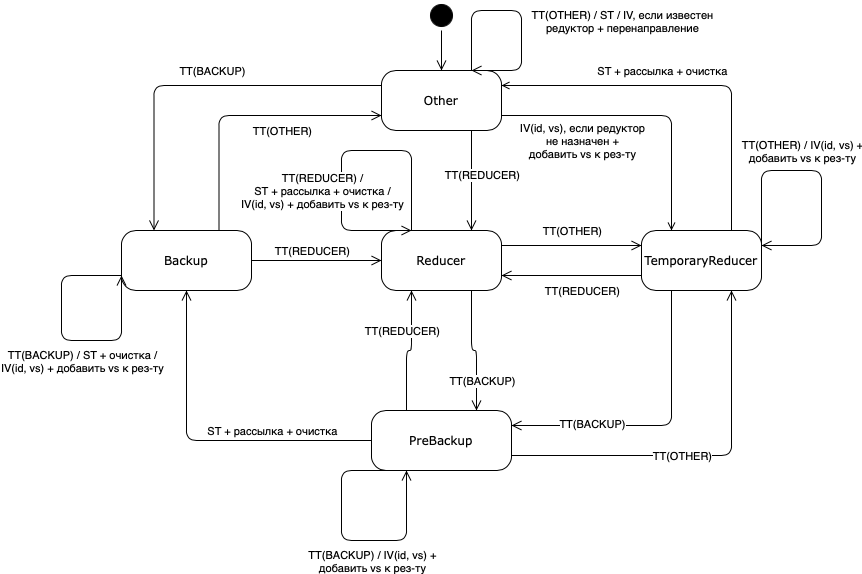
\includegraphics[scale=0.45]{images/NeighbourStateMachine_rus.png}
\captionsetup{justification=centering}
\caption{Состояния автомата и переходы в нем.}
\label{StateMachineImage}
\end{figure}

Разберем по отдельности каждое из упомянутых состояний: какой эффект вызывает обработка различных событий, в какие другие состояния оно может перейти.

\subsubsection{Состояние ReducerState}

ReducerState -- состояние по умолчанию для узла, выбранного в качестве редуктора в пределах группы. Находясь в этом состоянии, узел агрегирует значения приходящих индивидуальных счетчиков от узлов его группы для получения результата локальной редукции, а также регулярно рассылает накопленный результат по узлам всей системы. Приходящие события в этом состоянии обрабатываются следующим образом:

\begin{itemize}
    \item IndividualValues(id, values): если битовая маска результата на месте id содержит $0$, значения счетчиков values добавляются в текущий результат редукции по обычному механизму, описанному в подразделе \ref{ReductionImplementationSubsection};
    
    \item TransitionTo(state): в зависимости от значения state происходит один из переходов:
        
        \begin{itemize}
            \item \texttt{REDUCER}: событие игнорируется (узел уже находится в нужном состоянии);
            \item \texttt{BACKUP\_REDUCER}: совершается переход в состояние PreBackupState;
            \item \texttt{OTHER}: совершается переход в состояние TemporaryReducerState;
        \end{itemize}
        
    \item ScatterTimeout: текущий накопленный результат локальной редукции рассылается по всем узлам системы с помощью операции scatter, а затем очищается.
\end{itemize}

Соответствующая реализация интерфейса \texttt{State} представлена в листинге \ref{lst:ReducerStateImplementation}.

\begin{listing}[!htb]
\begin{minted}
[
frame=lines,
framesep=2mm,
baselinestretch=1.2,
fontsize=\normalsize,
linenos
]
{python}
class ReducerState(State):
    def __init__(self) -> None:
        super().__init__()

    def handle_individual_values(self, individual_values: IndividualValues) -> None:
        if self.context is not None:
            self.context.local_reducer.add_individual_values(individual_values)

    def handle_state_transition(self, to_state: NeighbourState.V) -> None:
        if to_state == REDUCER or self.context is None:
            return
        elif to_state == BACKUP_REDUCER:
            self.context.transition_to(PreBackupState())
        elif to_state == OTHER:
            self.context.transition_to(TemporaryReducerState())

    def handle_scatter_timeout(self) -> None:
        if self.context is not None:
            self.context.scatter_reduction_result()
            self.context.local_reducer.clear_reduction_result()
\end{minted}
\caption{Реализация класса \texttt{ReducerState}, соответствующая состоянию ReducerState.}
\label{lst:ReducerStateImplementation}
\end{listing}

\subsubsection{Состояние BackupState}

BackupState -- состояние по умолчанию для узла, выбранного в качестве резервного редуктора в пределах площадки. Работа узла в данном состоянии аналогична работе в состоянии ReducerState с тем лишь отличием, что при обработке события ScatterTimeout он не рассылает накопленный результат, а просто очищает текущий. Обработка события TransitionTo(state) также отличается:

\begin{itemize}
    \item Если state равно \texttt{BACKUP\_REDUCER}, событие игнорируется;
    \item Если state равно \texttt{REDUCER}, то совершается переход в ReducerState;
    \item Если state равно \texttt{OTHER}, накопленный результат редукции очищается, совершается переход в OtherState.
\end{itemize}

Реализация интерфейса представлена в листинге \ref{lst:BackupStateImplementation}.

\begin{listing}[!htb]
\begin{minted}
[
frame=lines,
framesep=2mm,
baselinestretch=1.2,
fontsize=\normalsize,
linenos
]
{python}
class BackupState(State):
    def __init__(self) -> None:
        super().__init__()

    def handle_individual_values(self, individual_values: IndividualValues) -> None:
        if self.context is not None:
            self.context.local_reducer.add_individual_values(individual_values)

    def handle_state_transition(self, to_state: NeighbourState.V) -> None:
        if to_state == BACKUP_REDUCER or self.context is None:
            return
        elif to_state == REDUCER:
            self.context.transition_to(ReducerState())
        elif to_state == OTHER:
            self.context.local_reducer.clear_reduction_result()
            self.context.transition_to(OtherState())

    def handle_scatter_timeout(self) -> None:
        if self.context is not None:
            self.context.local_reducer.clear_reduction_result()
\end{minted}
\caption{Реализация класса \texttt{BackupState}, соответствующая состоянию BackupState.}
\label{lst:BackupStateImplementation}
\end{listing}

Данное состояние, как и общая идея резервного редуктора, предназначено для быстрой смены редуктора: с момента отказа последнего до момента явной смены состояния он будет продолжать накапливать значение локальной редукции, поэтому при становлении редуктором ему не придется агрегировать все данные с нуля.

\subsubsection{Состояние OtherState}

OtherState -- состояние по умолчанию узла, не являющегося ни редуктором, ни резервным редуктором. События в нем обрабатываются следующим образом:

\begin{itemize}
    \item IndividualValues(id, values): если текущий узел считает редуктором один из узлов площадки, полученное сообщение с индивидуальными счетчиками перенаправляется данному узлу, иначе совершается переход в состояние TemporaryReducerState, и то же событие обрабатывается в новом состоянии;
    
    \item TransitionTo(state): в зависимости от значения state происходит один из переходов:
        
        \begin{itemize}
            \item \texttt{OTHER}: событие игнорируется;
            \item \texttt{BACKUP\_REDUCER}: совершается переход в состояние BackupState;
            \item \texttt{REDUCER}: совершается переход в состояние ReducerState;
        \end{itemize}
        
    \item ScatterTimeout: событие игнорируется.
\end{itemize}

Код реализации данного состояния представлен в листинге \ref{lst:OtherStateImplementation}.

\begin{listing}[!htb]
\begin{minted}
[
frame=lines,
framesep=2mm,
baselinestretch=1.2,
fontsize=\normalsize,
linenos
]
{python}
class OtherState(State):
    def __init__(self) -> None:
        super().__init__()

    def handle_individual_values(self, individual_values: IndividualValues) -> None:
        if self.context is None:
            return
        if self.context.designator is None or \
                self.context.designator.get_reducer() < 0 or \
                individual_values.ttl <= 0:
            self.context.transition_to(TemporaryReducerState())
            self.context.handle_individual_values(individual_values)
        else:
            individual_values.ttl -= 1
            self.context.local_sender.send_individual_values(
                individual_values,
                self.context.designator.get_reducer()
            )

    def handle_state_transition(self, to_state: NeighbourState.V) -> None:
        if to_state == OTHER or self.context is None:
            return
        elif to_state == REDUCER:
            self.context.transition_to(ReducerState())
        elif to_state == BACKUP_REDUCER:
            self.context.transition_to(BackupState())
\end{minted}
\caption{Реализация класса \texttt{OtherState}, соответствующая состоянию OtherState.}
\label{lst:OtherStateImplementation}
\end{listing}

Стоит отметить, что здесь мы также применяем подход с добавлением к сообщениям TTL-поля, поскольку мы не можем с уверенностью заверять, что циклов при выборе редуктора не образуется.

Как мы помним, при реализации алгоритма выбора редуктора и резервного редуктора мы пожертвовали согласованностью выбора в пользу доступности. Тем не менее, с помощью описанных перенаправлений сообщений и раннего вхождения в состояние TemporaryReducerState мы можем компенсировать несогласованный выбор. Последние два состояния, которые мы опишем в подразделах \ref{TemporaryReducerStateSubsection} и \ref{PreBackupStateSubsection} также предназначены для того, чтобы бороться с проблемой несогласованного выбора редуктора.

\subsubsection{Состояние TemporaryReducerState}
\label{TemporaryReducerStateSubsection}

TemporaryReducerState -- состояние узла, который уже (или еще) не является редуктором, но у которого есть некоторый результат редукции, который может быть необходим для формирования корректного результата глобальной редукции. В это состояние может переходить редуктор с меньшим идентификатором узла при возникновении конфликтов или узел, который еще не успел узнать, кто на площадке является редуктором. При этом мы считаем, что данное состояние временное: коль скоро узел сам не является редуктором, однажды другие узлы перестанут считать его таковым, поэтому при следующем срабатывании таймера, которое породит событие ScatterTimeout, данный узел инициирует рассылку своего результата редукции, а затем перейдет в стандартное состояние OtherState. Итак, опишем его действия при при обработке всевозможных событий:

\begin{itemize}
    \item IndividualValues(id, values): индивидуальные счетчики добавляются к текущему результату редукции по обычному механизму, описанному в подразделе \ref{ReductionImplementationSubsection};
    
    \item TransitionTo(state): в зависимости от значения state происходит один из переходов:
        
        \begin{itemize}
            \item \texttt{OTHER}: событие игнорируется;
            \item \texttt{BACKUP\_REDUCER}: совершается переход в состояние PreBackupState;
            \item \texttt{REDUCER}: совершается переход в состояние ReducerState;
        \end{itemize}
        
    \item ScatterTimeout: текущий накопленный результат локальной редукции рассылается по всем узлам системы с помощью операции scatter, а затем очищается, совершается переход в состояние OtherState.
\end{itemize}

На листинге \ref{lst:TemporaryReducerStateImplementation} представлен код реализации состояния TemporaryReducerState.

\begin{listing}[!htb]
\begin{minted}
[
frame=lines,
framesep=2mm,
baselinestretch=1.2,
fontsize=\normalsize,
linenos
]
{python}
class TemporaryReducerState(State):
    def __init__(self) -> None:
        super().__init__()

    def handle_individual_values(self, individual_values: IndividualValues) -> None:
        if self.context is not None:
            self.context.local_reducer.add_individual_values(individual_values)

    def handle_state_transition(self, to_state: NeighbourState.V) -> None:
        if to_state == OTHER or self.context is None:
            return
        elif to_state == REDUCER:
            self.context.transition_to(ReducerState())
        elif to_state == BACKUP_REDUCER:
            self.context.transition_to(PreBackupState())

    def handle_scatter_timeout(self) -> None:
        if self.context is not None:
            self.context.scatter_reduction_result(True)
            self.context.local_reducer.clear_reduction_result()
            self.context.transition_to(OtherState())
\end{minted}
\caption{Реализация класса \texttt{TemporaryReducerState}, соответствующая состоянию TemporaryReducerState.}
\label{lst:TemporaryReducerStateImplementation}
\end{listing}

\subsubsection{Состояние PreBackupState}
\label{PreBackupStateSubsection}

Состояние PreBackupState аналогично состоянию TemporaryReducerState с теми лишь отличиями, что по истечениии таймера переход совершается в состояние Ba\-ckup\-State, и переходы при обработке событий TransitionTo отличаются ввиду того, что узел, находящийся в данном состоянии является резервным редуктором на площадке в терминах алгоритма выбора \ref{ReducersElectionSubsection}. Для наглядности опустим описание действий при обработке каждого события, а лишь приложим код реализации (листинг \ref{lst:PreBackupStateImplementation}).

\begin{listing}[!htb]
\begin{minted}
[
frame=lines,
framesep=2mm,
baselinestretch=1.2,
fontsize=\normalsize,
linenos
]
{python}
class PreBackupState(State):
    def __init__(self) -> None:
        super().__init__()

    def handle_individual_values(self, individual_values: IndividualValues) -> None:
        if self.context is not None:
            self.context.local_reducer.add_individual_values(individual_values)

    def handle_state_transition(self, to_state: NeighbourState.V) -> None:
        if to_state == BACKUP_REDUCER or self.context is None:
            return
        elif to_state == REDUCER:
            self.context.transition_to(ReducerState())
        elif to_state == OTHER:
            self.context.transition_to(TemporaryReducerState())

    def handle_scatter_timeout(self) -> None:
        if self.context is not None:
            self.context.scatter_reduction_result(True)
            self.context.local_reducer.clear_reduction_result()
            self.context.transition_to(BackupState())
\end{minted}
\caption{Реализация класса \texttt{PreBackupState}, соответствующая состоянию PreBackupState.}
\label{lst:PreBackupStateImplementation}
\end{listing}

Описав работу автомата состояний, а также механизм, по которому выполняются локальные и глобальные редукции, мы завершили построение общего алгоритма выполнения операции AllReduce. Для того, чтобы мы могли судить о качестве предложенного решения, опишем и докажем его свойства в следующем разделе \ref{AllReduceCorrectnessSection}.

\section{Корректность реализации AllReduce}
\label{AllReduceCorrectnessSection}

В данном разделе опишем и докажем гарантии на корректность выполнения операции AllReduce, которые удалось достичь, построив предложенный дизайн системы.

\begin{theorem}
\label{ConsistentStateCorrectness}
    Пусть с момента времени $t_0 \in T$ выбор редукторов на каждой из площадок согласован, узлы не отказывают, все сообщения в сети доставляются, а время задержек при выполнении операции scatter составляет не более $\Delta_w$, т.е. рассылаемые данные дойдут до всех узлов системы не позднее, чем через $\Delta_w$ времени после инициирования рассылки. При этом будем считать, что интервалы таймеров $\Delta_{iv}$, $\Delta_s$, а также задержки на передачу данных между узлами одной площадки таковы, что за любой промежуток времени $\Delta_s$ редуктор успевает получить данные индивидуальных счетчиков каждого другого рабочего узла площадки. Тогда переданный потребителю глобальный результат редукции на любом узле в момент времени $t > t_0 + \Delta_f + 2\Delta_w + \Delta_s$ будет являться корректным результатом выполнения операции AllReduce с допустимым временным отклонением в $\Delta_f + 2\Delta_w + \Delta_s$.
\end{theorem}
\begin{proof}
    Из условия теоремы следует, что любой результат локальной редукции при рассылке будет содержать данные всех работающих узлов на площадке за последний интервал времени в $\Delta_s$. Это в свою очередь означает, что при истечении таймера в $\Delta_f$ времени результат глобальной редукции на узле может быть не передан потребителю из-за неполной битовой маски лишь в 2 случаях: 1) некоторый узел отказал, поэтому локальная редукция с его площадки не содержала соответсвтующий единичный бит в маске; 2) из-за задержек сети за последний отрезок времени в $\Delta_f$ результат локальной редукции с некоторой группы еще не успел дойти до текущего узла. Если все узлы системы находились в рабочем состоянии, возможен лишь второй случай, поскольку интервал рассылки результата локальной редукции $\Delta_s$ не больше интервала $\Delta_f$, после которого результат глобальной редукции проверяется на полноту, а значит за время последней итерации подсчета глобальной редукции результаты локальных редукций всех групп были отправлены хотя бы один раз, и, коль скоро все сообщения по условию доставляются, они еще не были доставлены лишь из-за возникших задержек.
    
    Итак, передача результата глобальной редукции потребителю в момент времени $t$ могла произойти в 3 случаях. Разберем их далее.
    
    \begin{enumerate}
        \item Передача потребителю произошла после истечения таймера в $\Delta_f$ времени. Это стандартная ситуация, в этом случае битовая маска состоит лишь из единичных битов, а значит результат содержит данные счетчиков всех узлов системы, при этом ни один из них не был учтен дважды -- из рассуждений выше результаты локальных редукций имели одинаковые битовые маски, а значит ни один из них не мог добавиться в глобальную редукцию дважды. Мы также знаем, что в момент времени $t - \Delta_f$ результат глобальной редукции на узле был очищен, а значит в итоговый результат могли попасть лишь те значения локальных редукций, которые были отправлены не раньше $t - \Delta_f - \Delta_w$ -- из условия на время задержек. Накопление результата локальной редукции длится $\Delta_s$ времени. Таким образом, результат глобальной редукции, переданный потребителю в момент времени $t$, содержал в себе значения счетчиков всех узлов, каждый из которых присутствовал на соответствующем узле не более $\Delta_f + \Delta_w + \Delta_s$ времени назад относительно $t$. В данном случае теорема доказана.
        
        \item Передача потребителю произошла из отложенного результата глобальной редукции \texttt{waiting\_result} после того, как было получено очередное сообщение с результатом локальной редукции и битовая маска отложенного результата стала состоять из единичных битов. Это могло произойти не позже, чем через $\Delta_w$ времени после очередного срабатывания таймера в $\Delta_f$ времени -- иначе текущий отложенный результат передался бы потребителю даже без полной битовой маски. Поэтому, проведя рассуждения, аналогичные предыдущему пункту, мы можем заключить, что такой отложенный результат будет содержать значения счетчиков, присутствовавших на узлах не раньше момента времени $t - \Delta_f - 2\Delta_w - \Delta_s$. Аналогично, теорема доказана.
        
        \item Передача потребителю отложенного результата глобальный редукции произошла по истечению таймера в $\Delta_w$ времени. Однако из проведенных ранее рассуждений такого не могло произойти: на момент срабатывания таймера в $\Delta_f$ времени все результаты локальных редукций были уже либо учтены в глобальной редукции, либо отправлены, а, коль скоро задрежки при рассылке не превосходят $\Delta_w$, до срабатывания соответствующего таймера данные должны были дойти и учесться в отложенном результате.
    \end{enumerate}
    
    Таким образом, во всех возможных случаях передачи результата глобальной редукции потребителю условия на его корректность из формулировки теоремы выполняются, поэтому теорему можно считать доказанной.
\end{proof}

\begin{consequence}
    Пусть с момента времени $t \in T$ узлы системы не отказывали. Тогда при соблюдении ограничений на качество сети из леммы \ref{ElectionEC} и теоремы \ref{ConsistentStateCorrectness} наступит момент времени $t_1 > t$ такой, что начиная с него результаты выполнения операции AllReduce будут корректны с допустимым временным отклонением в $\Delta_f + 2\Delta_w + \Delta_s$, причем $t_1 - t \leq \Delta_f + 2\Delta_w + \Delta_s + \Delta_{delay} + 9\Delta_{dead}$.
\end{consequence}
\begin{proof}
    По теореме \ref{ElectionLiveness} в течение времени $\Delta_{delay} + 9\Delta_{dead}$ после $t$ на каждой площадке редуктор будет выбран согласовано. Значит к моменту времени $t + \Delta_{delay} + 9\Delta_{dead}$ можно применить утверждение теоремы \ref{ConsistentStateCorrectness}. В итоге получим, что начиная с момента времени $t + \Delta_f + 2\Delta_w + \Delta_s + \Delta_{delay} + 9\Delta_{dead}$ гарантировано все результаты выполнения операции AllReduce будут корректны с допустимым временным отклонением в $\Delta_f + 2\Delta_w + \Delta_s$.
\end{proof}

\begin{consequence}
    Пусть непосредственно до момента времени $t \in T$ в пределах каждой площадки выбор редуктора и резервного редуктора был согласован, а в момент времени $t$ на одной или нескольких площадках назначенный редуктор отказал. Пусть при этом после момента времени $t$ узлы не отказывали, и выполнялись все условия на качество сети из теорем \ref{ReelectionTheorem} и \ref{ConsistentStateCorrectness}. Тогда любой результат глобальной редукции, переданный потребителю в момент времени $t_1 > t + \Delta_{delay} + 2\Delta_{dead} + \Delta_f + 2\Delta_w + \Delta_s$, будет являться корректным результатом выполнения операции AllReduce с допустимым временным отклонением $\Delta_f + 2\Delta_w + \Delta_s$.
\end{consequence}
\begin{proof}
    Коль скоро выбор редуктора и резервного редуктора в пределах каждой площадки до момента $t$ был согласован, то по теореме \ref{ReelectionTheorem} в течение следующего отрезка в $\Delta_{delay} + 2\Delta_{dead}$ времени на каждой площадке, в которой отказали назначенные редукторы, в качестве нового редуктора будет выбран резервный редуктор. Поэтому мы можем применить утверждение теоремы \ref{ConsistentStateCorrectness} к моменту времени $t + \Delta_{delay} + 2\Delta_{dead}$ и получить требуемое.
\end{proof}

Итого, сформулировав и доказав перечисленные свойства алгоритма, мы можем утверждать, что построили решение, удовлетворяющее поставленным требованиям: при его использовании операция AllReduce завершается корректно, при этом вся система способна переживать отказы и за ограниченное время возвращаться к штатному режиму работы. Можем переходить к перечислению результатов работы и выводам.

\section{Заключение}

\subsection{Результаты}

В процессе работы над исходной задачей мы подробно изучили ее проблематику и сумели выработать подходящее решение, которое удовлетворяет поставленным требованиям. Мы также получили ряд полезных результатов по теме работы:

\begin{itemize}
    \item рассмотрели различные подходы к реализации операции AllReduce, в том числе с применением готовых инструментов, таких, как: интерфейс MPI и согласованное в конечном счете хранилище;
    
    \item выработали концепцию решения, использующую идею частичных редукций, которая позволила снизить потребляемые ресурсы системы на хранение и обмен данными счетчиков;
    
    \item реализовали алгоритм выбора узлов для промежуточных редукций и доказали, что выбор становится согласованным за ограниченный отрезок времени;
    
    \item построили протокол маршрутизации на уровне узлов системы, позволяющий передавать данные по эффективным с точки зрения суммарной метрики маршрутам, а также доказали, что алгоритм маршрутизации в конечном счете строит наилучшие маршруты;
    
    \item описали алгоритм выполнения операции AllReduce, использующий метод проведения частичных редукций на узлах-редукторах и автомат состояний, определяющий эффект от событий различного типа;
    
    \item доказали, что при соблюдении определенных условий на качество сети предложенная реализация AllReduce корректна, а также то, что при единичных отказах оборудования алгоритм продолжает работать и за ограниченное время снова начинает выдавать корректный результат редукции;
    
    \item реализовали основные части системы в виде прототипа на языке Python (приложение \ref{GitHubLinkAppendix}).
\end{itemize}

\subsection{Выводы}

В данной работе была рассмотрена операция AllReduce и ее реализация в рамках системы, обладающей специфичной топологией сети, которой зачастую обладают инфраструктуры компаний, предоставляющих геораспределенные облачные сервисы. Нам удалось предложить более эффективное решение по сравнению с наивным подходом. В основе данного решения лежат две основных оптимизации: подсчет промежуточных редукций и построение наилучших маршрутов в сети. Мы также показали, что алгоритм продолжает свою работу при отказах узлов. Таким образом, нам удалось достичь поставленной цели: мы снизили стоимость передачи данных между узлами системы и обеспечили определенный уровень отказоустойчивости.

\subsection{Дальнейшая работа}

Несмотря на большой объем проделанной работы, тема исследования содержит ряд особенностей для дальнейшего изучения.

Во-первых, стоит отметить, что большая часть данной работы была посвящена теоретической стороне вопроса, а также проектированию общего дизайна системы. Поэтому для того, чтобы полностью убедиться в работоспособности описанной системы, в будущем предстоит провести тестирование в лабораторных условиях, а также на данных, приближенных к реальным. При этом прототип системы, реализованный нами на языке Python, может послужить отправной точкой для дальнейшей разработки готового продукта.

Во-вторых, говоря о внедрении проекта в реальную инфраструктуру той или иной компании, не стоит упускать такую деталь реализации, как конфигурация системы. В данной работе мы абстрагировались от задачи введения новых узлов сети в работу и вывода из нее. Мы считали, что все узлы друг про друга знают: в простейшем случае это настраивается статически, а для более продвинутого варианта необходимо разрабатывать отдельный протокол, по которому они будут получать информацию о соседях динамически. Тем не менее, при реализации готовой системы этот аспект должен быть учтен.

В конце концов, при необходимости за счет введения дополнительных сущностей и механизмов можно постараться улучшить наше решение с точки зрения качества результата глобальной редукции. Мы показали, что при наложении разумных условий на задержки в сети получаемый результат операции AllReduce корректен с ограниченным допустимым временным отклонением. Если полученную оценку удасться уменьшить с помощью надстроек, это позволит улучшить работу всего алгоритма.

\clearpage

\bibliographystyle {unsrt}
\bibliography{refs.bib}

\clearpage

\begin{appendices}
\titleformat{\section}[display]
  {\normalfont\Large\bfseries}
  {\centering ПРИЛОЖЕНИЕ}
  {0pt}{\Large\centering}
\renewcommand{\thesection}{\Asbuk{section}}

\section{Ссылка на репозиторий с кодом проекта}
\label{GitHubLinkAppendix}
\url{https://github.com/regu1yar/qnet-bachelor-thesis}
\end{appendices}

\end{document}
